% Options for packages loaded elsewhere
\PassOptionsToPackage{unicode}{hyperref}
\PassOptionsToPackage{hyphens}{url}
%
\documentclass[
]{article}
\usepackage{amsmath,amssymb}
\usepackage{iftex}
\ifPDFTeX
  \usepackage[T1]{fontenc}
  \usepackage[utf8]{inputenc}
  \usepackage{textcomp} % provide euro and other symbols
\else % if luatex or xetex
  \usepackage{unicode-math} % this also loads fontspec
  \defaultfontfeatures{Scale=MatchLowercase}
  \defaultfontfeatures[\rmfamily]{Ligatures=TeX,Scale=1}
\fi
\usepackage{lmodern}
\ifPDFTeX\else
  % xetex/luatex font selection
\fi
% Use upquote if available, for straight quotes in verbatim environments
\IfFileExists{upquote.sty}{\usepackage{upquote}}{}
\IfFileExists{microtype.sty}{% use microtype if available
  \usepackage[]{microtype}
  \UseMicrotypeSet[protrusion]{basicmath} % disable protrusion for tt fonts
}{}
\makeatletter
\@ifundefined{KOMAClassName}{% if non-KOMA class
  \IfFileExists{parskip.sty}{%
    \usepackage{parskip}
  }{% else
    \setlength{\parindent}{0pt}
    \setlength{\parskip}{6pt plus 2pt minus 1pt}}
}{% if KOMA class
  \KOMAoptions{parskip=half}}
\makeatother
\usepackage{xcolor}
\usepackage[margin=1in]{geometry}
\usepackage{color}
\usepackage{fancyvrb}
\newcommand{\VerbBar}{|}
\newcommand{\VERB}{\Verb[commandchars=\\\{\}]}
\DefineVerbatimEnvironment{Highlighting}{Verbatim}{commandchars=\\\{\}}
% Add ',fontsize=\small' for more characters per line
\usepackage{framed}
\definecolor{shadecolor}{RGB}{248,248,248}
\newenvironment{Shaded}{\begin{snugshade}}{\end{snugshade}}
\newcommand{\AlertTok}[1]{\textcolor[rgb]{0.94,0.16,0.16}{#1}}
\newcommand{\AnnotationTok}[1]{\textcolor[rgb]{0.56,0.35,0.01}{\textbf{\textit{#1}}}}
\newcommand{\AttributeTok}[1]{\textcolor[rgb]{0.13,0.29,0.53}{#1}}
\newcommand{\BaseNTok}[1]{\textcolor[rgb]{0.00,0.00,0.81}{#1}}
\newcommand{\BuiltInTok}[1]{#1}
\newcommand{\CharTok}[1]{\textcolor[rgb]{0.31,0.60,0.02}{#1}}
\newcommand{\CommentTok}[1]{\textcolor[rgb]{0.56,0.35,0.01}{\textit{#1}}}
\newcommand{\CommentVarTok}[1]{\textcolor[rgb]{0.56,0.35,0.01}{\textbf{\textit{#1}}}}
\newcommand{\ConstantTok}[1]{\textcolor[rgb]{0.56,0.35,0.01}{#1}}
\newcommand{\ControlFlowTok}[1]{\textcolor[rgb]{0.13,0.29,0.53}{\textbf{#1}}}
\newcommand{\DataTypeTok}[1]{\textcolor[rgb]{0.13,0.29,0.53}{#1}}
\newcommand{\DecValTok}[1]{\textcolor[rgb]{0.00,0.00,0.81}{#1}}
\newcommand{\DocumentationTok}[1]{\textcolor[rgb]{0.56,0.35,0.01}{\textbf{\textit{#1}}}}
\newcommand{\ErrorTok}[1]{\textcolor[rgb]{0.64,0.00,0.00}{\textbf{#1}}}
\newcommand{\ExtensionTok}[1]{#1}
\newcommand{\FloatTok}[1]{\textcolor[rgb]{0.00,0.00,0.81}{#1}}
\newcommand{\FunctionTok}[1]{\textcolor[rgb]{0.13,0.29,0.53}{\textbf{#1}}}
\newcommand{\ImportTok}[1]{#1}
\newcommand{\InformationTok}[1]{\textcolor[rgb]{0.56,0.35,0.01}{\textbf{\textit{#1}}}}
\newcommand{\KeywordTok}[1]{\textcolor[rgb]{0.13,0.29,0.53}{\textbf{#1}}}
\newcommand{\NormalTok}[1]{#1}
\newcommand{\OperatorTok}[1]{\textcolor[rgb]{0.81,0.36,0.00}{\textbf{#1}}}
\newcommand{\OtherTok}[1]{\textcolor[rgb]{0.56,0.35,0.01}{#1}}
\newcommand{\PreprocessorTok}[1]{\textcolor[rgb]{0.56,0.35,0.01}{\textit{#1}}}
\newcommand{\RegionMarkerTok}[1]{#1}
\newcommand{\SpecialCharTok}[1]{\textcolor[rgb]{0.81,0.36,0.00}{\textbf{#1}}}
\newcommand{\SpecialStringTok}[1]{\textcolor[rgb]{0.31,0.60,0.02}{#1}}
\newcommand{\StringTok}[1]{\textcolor[rgb]{0.31,0.60,0.02}{#1}}
\newcommand{\VariableTok}[1]{\textcolor[rgb]{0.00,0.00,0.00}{#1}}
\newcommand{\VerbatimStringTok}[1]{\textcolor[rgb]{0.31,0.60,0.02}{#1}}
\newcommand{\WarningTok}[1]{\textcolor[rgb]{0.56,0.35,0.01}{\textbf{\textit{#1}}}}
\usepackage{graphicx}
\makeatletter
\def\maxwidth{\ifdim\Gin@nat@width>\linewidth\linewidth\else\Gin@nat@width\fi}
\def\maxheight{\ifdim\Gin@nat@height>\textheight\textheight\else\Gin@nat@height\fi}
\makeatother
% Scale images if necessary, so that they will not overflow the page
% margins by default, and it is still possible to overwrite the defaults
% using explicit options in \includegraphics[width, height, ...]{}
\setkeys{Gin}{width=\maxwidth,height=\maxheight,keepaspectratio}
% Set default figure placement to htbp
\makeatletter
\def\fps@figure{htbp}
\makeatother
\setlength{\emergencystretch}{3em} % prevent overfull lines
\providecommand{\tightlist}{%
  \setlength{\itemsep}{0pt}\setlength{\parskip}{0pt}}
\setcounter{secnumdepth}{-\maxdimen} % remove section numbering
\ifLuaTeX
  \usepackage{selnolig}  % disable illegal ligatures
\fi
\usepackage{bookmark}
\IfFileExists{xurl.sty}{\usepackage{xurl}}{} % add URL line breaks if available
\urlstyle{same}
\hypersetup{
  pdftitle={DATA 621 HW4 WA},
  pdfauthor={Warner Alexis, Saloua Daouki, Souleymane Doumbia, Fomba Kassoh, Lewris Mota Sanchez},
  hidelinks,
  pdfcreator={LaTeX via pandoc}}

\title{DATA 621 HW4 WA}
\author{Warner Alexis, Saloua Daouki, Souleymane Doumbia, Fomba Kassoh,
Lewris Mota Sanchez}
\date{2024-11-17}

\begin{document}
\maketitle

{
\setcounter{tocdepth}{3}
\tableofcontents
}
\subsection{Introduction}\label{introduction}

The objective is to build two models using the provided dataset: a
multiple linear regression model to predict the cost of a car crash (a
continuous variable) and a binary logistic regression model to predict
the probability of a car crash (a binary outcome). Only the given
variables, or any new variables derived from them, can be used to build
these models. The dataset includes a set of variables relevant to the
prediction task, which are described in the following section.

\begin{figure}
\centering
\includegraphics{C:/Users/Warner_Beast/OneDrive/Documents/CUNY/DATA 621 - Data Mining/week 12/Screenshot 2024-11-17 122322.png}
\caption{Project Data}
\end{figure}

\begin{Shaded}
\begin{Highlighting}[]
\FunctionTok{library}\NormalTok{(dplyr)}
\end{Highlighting}
\end{Shaded}

\begin{verbatim}
## 
## Attaching package: 'dplyr'
\end{verbatim}

\begin{verbatim}
## The following objects are masked from 'package:stats':
## 
##     filter, lag
\end{verbatim}

\begin{verbatim}
## The following objects are masked from 'package:base':
## 
##     intersect, setdiff, setequal, union
\end{verbatim}

\begin{Shaded}
\begin{Highlighting}[]
\FunctionTok{library}\NormalTok{(ggplot2)}
\FunctionTok{library}\NormalTok{(DataExplorer)}
\FunctionTok{library}\NormalTok{(caret)}
\end{Highlighting}
\end{Shaded}

\begin{verbatim}
## Loading required package: lattice
\end{verbatim}

\begin{Shaded}
\begin{Highlighting}[]
\FunctionTok{library}\NormalTok{(car)}
\end{Highlighting}
\end{Shaded}

\begin{verbatim}
## Loading required package: carData
\end{verbatim}

\begin{verbatim}
## 
## Attaching package: 'car'
\end{verbatim}

\begin{verbatim}
## The following object is masked from 'package:dplyr':
## 
##     recode
\end{verbatim}

\begin{Shaded}
\begin{Highlighting}[]
\FunctionTok{library}\NormalTok{(e1071)}
\FunctionTok{library}\NormalTok{(MASS)}
\end{Highlighting}
\end{Shaded}

\begin{verbatim}
## 
## Attaching package: 'MASS'
\end{verbatim}

\begin{verbatim}
## The following object is masked from 'package:dplyr':
## 
##     select
\end{verbatim}

\begin{Shaded}
\begin{Highlighting}[]
\FunctionTok{library}\NormalTok{(pROC)}
\end{Highlighting}
\end{Shaded}

\begin{verbatim}
## Type 'citation("pROC")' for a citation.
\end{verbatim}

\begin{verbatim}
## 
## Attaching package: 'pROC'
\end{verbatim}

\begin{verbatim}
## The following objects are masked from 'package:stats':
## 
##     cov, smooth, var
\end{verbatim}

\begin{Shaded}
\begin{Highlighting}[]
\FunctionTok{library}\NormalTok{(VIM)}
\end{Highlighting}
\end{Shaded}

\begin{verbatim}
## Loading required package: colorspace
\end{verbatim}

\begin{verbatim}
## 
## Attaching package: 'colorspace'
\end{verbatim}

\begin{verbatim}
## The following object is masked from 'package:pROC':
## 
##     coords
\end{verbatim}

\begin{verbatim}
## Loading required package: grid
\end{verbatim}

\begin{verbatim}
## VIM is ready to use.
\end{verbatim}

\begin{verbatim}
## Suggestions and bug-reports can be submitted at: https://github.com/statistikat/VIM/issues
\end{verbatim}

\begin{verbatim}
## 
## Attaching package: 'VIM'
\end{verbatim}

\begin{verbatim}
## The following object is masked from 'package:datasets':
## 
##     sleep
\end{verbatim}

\subsection{Data Exploration}\label{data-exploration}

The training dataset consists of 8,161 observations and 26 variables.
Several categorical variables require transformation to be compatible
with both logistic and linear models. We begin with some fundamental
transformations.

\begin{verbatim}
## 'data.frame':    8161 obs. of  26 variables:
##  $ INDEX      : int  1 2 4 5 6 7 8 11 12 13 ...
##  $ TARGET_FLAG: int  0 0 0 0 0 1 0 1 1 0 ...
##  $ TARGET_AMT : num  0 0 0 0 0 ...
##  $ KIDSDRIV   : int  0 0 0 0 0 0 0 1 0 0 ...
##  $ AGE        : int  60 43 35 51 50 34 54 37 34 50 ...
##  $ HOMEKIDS   : int  0 0 1 0 0 1 0 2 0 0 ...
##  $ YOJ        : int  11 11 10 14 NA 12 NA NA 10 7 ...
##  $ INCOME     : chr  "$67,349" "$91,449" "$16,039" "" ...
##  $ PARENT1    : chr  "No" "No" "No" "No" ...
##  $ HOME_VAL   : chr  "$0" "$257,252" "$124,191" "$306,251" ...
##  $ MSTATUS    : chr  "z_No" "z_No" "Yes" "Yes" ...
##  $ SEX        : chr  "M" "M" "z_F" "M" ...
##  $ EDUCATION  : chr  "PhD" "z_High School" "z_High School" "<High School" ...
##  $ JOB        : chr  "Professional" "z_Blue Collar" "Clerical" "z_Blue Collar" ...
##  $ TRAVTIME   : int  14 22 5 32 36 46 33 44 34 48 ...
##  $ CAR_USE    : chr  "Private" "Commercial" "Private" "Private" ...
##  $ BLUEBOOK   : chr  "$14,230" "$14,940" "$4,010" "$15,440" ...
##  $ TIF        : int  11 1 4 7 1 1 1 1 1 7 ...
##  $ CAR_TYPE   : chr  "Minivan" "Minivan" "z_SUV" "Minivan" ...
##  $ RED_CAR    : chr  "yes" "yes" "no" "yes" ...
##  $ OLDCLAIM   : chr  "$4,461" "$0" "$38,690" "$0" ...
##  $ CLM_FREQ   : int  2 0 2 0 2 0 0 1 0 0 ...
##  $ REVOKED    : chr  "No" "No" "No" "No" ...
##  $ MVR_PTS    : int  3 0 3 0 3 0 0 10 0 1 ...
##  $ CAR_AGE    : int  18 1 10 6 17 7 1 7 1 17 ...
##  $ URBANICITY : chr  "Highly Urban/ Urban" "Highly Urban/ Urban" "Highly Urban/ Urban" "Highly Urban/ Urban" ...
\end{verbatim}

\begin{verbatim}
##      INDEX        TARGET_FLAG       TARGET_AMT        KIDSDRIV     
##  Min.   :    1   Min.   :0.0000   Min.   :     0   Min.   :0.0000  
##  1st Qu.: 2559   1st Qu.:0.0000   1st Qu.:     0   1st Qu.:0.0000  
##  Median : 5133   Median :0.0000   Median :     0   Median :0.0000  
##  Mean   : 5152   Mean   :0.2638   Mean   :  1504   Mean   :0.1711  
##  3rd Qu.: 7745   3rd Qu.:1.0000   3rd Qu.:  1036   3rd Qu.:0.0000  
##  Max.   :10302   Max.   :1.0000   Max.   :107586   Max.   :4.0000  
##                                                                    
##       AGE           HOMEKIDS           YOJ          INCOME         
##  Min.   :16.00   Min.   :0.0000   Min.   : 0.0   Length:8161       
##  1st Qu.:39.00   1st Qu.:0.0000   1st Qu.: 9.0   Class :character  
##  Median :45.00   Median :0.0000   Median :11.0   Mode  :character  
##  Mean   :44.79   Mean   :0.7212   Mean   :10.5                     
##  3rd Qu.:51.00   3rd Qu.:1.0000   3rd Qu.:13.0                     
##  Max.   :81.00   Max.   :5.0000   Max.   :23.0                     
##  NA's   :6                        NA's   :454                      
##    PARENT1            HOME_VAL           MSTATUS              SEX           
##  Length:8161        Length:8161        Length:8161        Length:8161       
##  Class :character   Class :character   Class :character   Class :character  
##  Mode  :character   Mode  :character   Mode  :character   Mode  :character  
##                                                                             
##                                                                             
##                                                                             
##                                                                             
##   EDUCATION             JOB               TRAVTIME        CAR_USE         
##  Length:8161        Length:8161        Min.   :  5.00   Length:8161       
##  Class :character   Class :character   1st Qu.: 22.00   Class :character  
##  Mode  :character   Mode  :character   Median : 33.00   Mode  :character  
##                                        Mean   : 33.49                     
##                                        3rd Qu.: 44.00                     
##                                        Max.   :142.00                     
##                                                                           
##    BLUEBOOK              TIF           CAR_TYPE           RED_CAR         
##  Length:8161        Min.   : 1.000   Length:8161        Length:8161       
##  Class :character   1st Qu.: 1.000   Class :character   Class :character  
##  Mode  :character   Median : 4.000   Mode  :character   Mode  :character  
##                     Mean   : 5.351                                        
##                     3rd Qu.: 7.000                                        
##                     Max.   :25.000                                        
##                                                                           
##    OLDCLAIM            CLM_FREQ        REVOKED             MVR_PTS      
##  Length:8161        Min.   :0.0000   Length:8161        Min.   : 0.000  
##  Class :character   1st Qu.:0.0000   Class :character   1st Qu.: 0.000  
##  Mode  :character   Median :0.0000   Mode  :character   Median : 1.000  
##                     Mean   :0.7986                      Mean   : 1.696  
##                     3rd Qu.:2.0000                      3rd Qu.: 3.000  
##                     Max.   :5.0000                      Max.   :13.000  
##                                                                         
##     CAR_AGE        URBANICITY       
##  Min.   :-3.000   Length:8161       
##  1st Qu.: 1.000   Class :character  
##  Median : 8.000   Mode  :character  
##  Mean   : 8.328                     
##  3rd Qu.:12.000                     
##  Max.   :28.000                     
##  NA's   :510
\end{verbatim}

\begin{verbatim}
##       INDEX TARGET_FLAG  TARGET_AMT    KIDSDRIV         AGE    HOMEKIDS 
##           0           0           0           0           6           0 
##         YOJ      INCOME     PARENT1    HOME_VAL     MSTATUS         SEX 
##         454           0           0           0           0           0 
##   EDUCATION         JOB    TRAVTIME     CAR_USE    BLUEBOOK         TIF 
##           0           0           0           0           0           0 
##    CAR_TYPE     RED_CAR    OLDCLAIM    CLM_FREQ     REVOKED     MVR_PTS 
##           0           0           0           0           0           0 
##     CAR_AGE  URBANICITY 
##         510           0
\end{verbatim}

The first graph displays the distribution of the \texttt{TARGET\_FLAG}
variable, which indicates whether a crash occurred (\texttt{1}) or did
not occur (\texttt{0}). The majority of observations fall into the ``No
Crash (0)'' category, with over 6,000 instances, while a smaller portion
represents the ``Crash (1)'' category. This suggests a significant class
imbalance in the dataset. To address this imbalance, techniques such as
resampling (oversampling the minority class or undersampling the
majority class) or weighted models may be necessary to prevent bias
toward the majority class.

The second graph provides an overview of missing data in the dataset.
The left plot illustrates the proportion of missing data for each
variable, showing that \texttt{CAR\_AGE} and \texttt{AGE} have the
highest proportion of missing data (around 6\% each), while most other
variables have little to no missing values. The right plot visualizes
the pattern of missing data, with red sections representing missing
values and blue sections indicating observed data. The missing data is
primarily concentrated in \texttt{CAR\_AGE} and \texttt{AGE}, while the
majority of the dataset is complete. To handle this, imputation
strategies such as replacing missing values with the mean or median, or
predictive imputation, can be employed. Alternatively, rows with missing
data can be excluded if they represent a small percentage of the
dataset. Proper handling of missing data is crucial for ensuring the
quality and reliability of the modeling process.

\begin{Shaded}
\begin{Highlighting}[]
\NormalTok{training\_data }\OtherTok{\textless{}{-}}\NormalTok{ insurance\_training}
\CommentTok{\# Missing Data Visualization}
\FunctionTok{aggr}\NormalTok{(training\_data, }\AttributeTok{col =} \FunctionTok{c}\NormalTok{(}\StringTok{\textquotesingle{}navyblue\textquotesingle{}}\NormalTok{, }\StringTok{\textquotesingle{}red\textquotesingle{}}\NormalTok{), }\AttributeTok{numbers =} \ConstantTok{TRUE}\NormalTok{, }\AttributeTok{sortVars =} \ConstantTok{TRUE}\NormalTok{, }\AttributeTok{labels =} \FunctionTok{names}\NormalTok{(training\_data), }
     \AttributeTok{cex.axis =} \FloatTok{0.7}\NormalTok{, }\AttributeTok{gap =} \DecValTok{3}\NormalTok{, }\AttributeTok{ylab =} \FunctionTok{c}\NormalTok{(}\StringTok{"Missing data"}\NormalTok{, }\StringTok{"Pattern"}\NormalTok{))}
\end{Highlighting}
\end{Shaded}

\includegraphics{Data-621-Hw4-Wa_files/figure-latex/unnamed-chunk-2-1.pdf}

\begin{verbatim}
## 
##  Variables sorted by number of missings: 
##     Variable       Count
##      CAR_AGE 0.062492342
##          YOJ 0.055630437
##          AGE 0.000735204
##        INDEX 0.000000000
##  TARGET_FLAG 0.000000000
##   TARGET_AMT 0.000000000
##     KIDSDRIV 0.000000000
##     HOMEKIDS 0.000000000
##       INCOME 0.000000000
##      PARENT1 0.000000000
##     HOME_VAL 0.000000000
##      MSTATUS 0.000000000
##          SEX 0.000000000
##    EDUCATION 0.000000000
##          JOB 0.000000000
##     TRAVTIME 0.000000000
##      CAR_USE 0.000000000
##     BLUEBOOK 0.000000000
##          TIF 0.000000000
##     CAR_TYPE 0.000000000
##      RED_CAR 0.000000000
##     OLDCLAIM 0.000000000
##     CLM_FREQ 0.000000000
##      REVOKED 0.000000000
##      MVR_PTS 0.000000000
##   URBANICITY 0.000000000
\end{verbatim}

\begin{Shaded}
\begin{Highlighting}[]
\CommentTok{\# Summary statistic }
\NormalTok{numeric\_vars }\OtherTok{\textless{}{-}}\NormalTok{ training\_data }\SpecialCharTok{\%\textgreater{}\%} \FunctionTok{select\_if}\NormalTok{(is.numeric)}
\FunctionTok{plot\_histogram}\NormalTok{(training\_data)}
\end{Highlighting}
\end{Shaded}

\includegraphics{Data-621-Hw4-Wa_files/figure-latex/unnamed-chunk-2-2.pdf}

\begin{Shaded}
\begin{Highlighting}[]
\NormalTok{DataExplorer}\SpecialCharTok{::}\FunctionTok{plot\_histogram}\NormalTok{(training\_data)}
\end{Highlighting}
\end{Shaded}

\includegraphics{Data-621-Hw4-Wa_files/figure-latex/unnamed-chunk-2-3.pdf}

\begin{Shaded}
\begin{Highlighting}[]
\FunctionTok{library}\NormalTok{(ggplot2)}
\CommentTok{\# Ananlyze response variables }
\CommentTok{\# Explore TARGET\_FLAG}
\FunctionTok{table}\NormalTok{(training\_data}\SpecialCharTok{$}\NormalTok{TARGET\_FLAG)}
\end{Highlighting}
\end{Shaded}

\begin{verbatim}
## 
##    0    1 
## 6008 2153
\end{verbatim}

\begin{Shaded}
\begin{Highlighting}[]
\FunctionTok{ggplot}\NormalTok{(training\_data, }\FunctionTok{aes}\NormalTok{(}\AttributeTok{x =} \FunctionTok{as.factor}\NormalTok{(TARGET\_FLAG))) }\SpecialCharTok{+}
  \FunctionTok{geom\_bar}\NormalTok{(}\AttributeTok{fill =} \StringTok{"skyblue"}\NormalTok{) }\SpecialCharTok{+}
  \FunctionTok{labs}\NormalTok{(}\AttributeTok{title =} \StringTok{"Distribution of TARGET\_FLAG"}\NormalTok{, }\AttributeTok{x =} \StringTok{"Crash (1) / No Crash (0)"}\NormalTok{, }\AttributeTok{y =} \StringTok{"Count"}\NormalTok{)}
\end{Highlighting}
\end{Shaded}

\includegraphics{Data-621-Hw4-Wa_files/figure-latex/unnamed-chunk-2-4.pdf}

\begin{Shaded}
\begin{Highlighting}[]
\CommentTok{\# Explore TARGET\_AMT}
\FunctionTok{ggplot}\NormalTok{(training\_data, }\FunctionTok{aes}\NormalTok{(}\AttributeTok{x =}\NormalTok{ TARGET\_AMT)) }\SpecialCharTok{+}
  \FunctionTok{geom\_histogram}\NormalTok{(}\AttributeTok{fill =} \StringTok{"darkgreen"}\NormalTok{, }\AttributeTok{bins =} \DecValTok{30}\NormalTok{) }\SpecialCharTok{+}
  \FunctionTok{labs}\NormalTok{(}\AttributeTok{title =} \StringTok{"Distribution of TARGET\_AMT"}\NormalTok{, }\AttributeTok{x =} \StringTok{"Cost of Crash"}\NormalTok{, }\AttributeTok{y =} \StringTok{"Count"}\NormalTok{) }\SpecialCharTok{+}
  \FunctionTok{xlim}\NormalTok{(}\DecValTok{0}\NormalTok{, }\FunctionTok{quantile}\NormalTok{(training\_data}\SpecialCharTok{$}\NormalTok{TARGET\_AMT, }\FloatTok{0.95}\NormalTok{))  }\CommentTok{\# Trim extreme outliers}
\end{Highlighting}
\end{Shaded}

\includegraphics{Data-621-Hw4-Wa_files/figure-latex/unnamed-chunk-2-5.pdf}

The graphic illustrates the relationship between several predictor
variables (e.g., ``Driving Children,'' ``Age of Driver'') and a target
variable, with the red line indicating trends in predicted
probabilities. Some variables, like ``Age of Driver,'' show a linear
relationship, as the probability decreases steadily with age. Others,
like ``Driving Children'' and ``Distance to Work,'' exhibit non-linear
trends, where the probability increases or changes in a curved manner.
For variables with linear relationships, no transformations are needed,
while non-linear relationships may require transformations (e.g.,
logarithmic or polynomial terms) or the use of splines to better capture
the trends. Additionally, interaction terms may be needed if
relationships between variables are interdependent. Finally, it is
essential to check for multicollinearity and reassess residuals after
modeling to ensure the relationships are accurately captured.

\begin{Shaded}
\begin{Highlighting}[]
\CommentTok{\# Correlation plot for numeric variables}
\FunctionTok{library}\NormalTok{(corrplot)}
\end{Highlighting}
\end{Shaded}

\begin{verbatim}
## corrplot 0.92 loaded
\end{verbatim}

\begin{Shaded}
\begin{Highlighting}[]
\NormalTok{corr\_matrix }\OtherTok{\textless{}{-}} \FunctionTok{cor}\NormalTok{(numeric\_vars, }\AttributeTok{use =} \StringTok{"complete.obs"}\NormalTok{)}
\FunctionTok{corrplot}\NormalTok{(corr\_matrix, }\AttributeTok{method =} \StringTok{"circle"}\NormalTok{, }\AttributeTok{type =} \StringTok{"lower"}\NormalTok{, }\AttributeTok{tl.col =} \StringTok{"black"}\NormalTok{, }\AttributeTok{tl.cex =} \FloatTok{0.7}\NormalTok{)}
\end{Highlighting}
\end{Shaded}

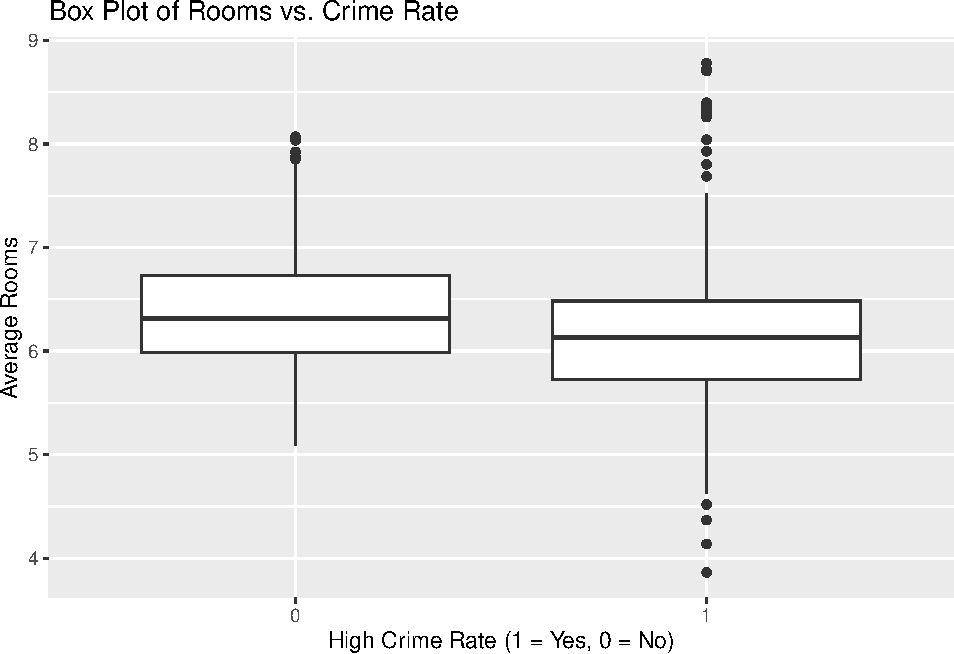
\includegraphics{Data-621-Hw4-Wa_files/figure-latex/unnamed-chunk-3-1.pdf}

\begin{Shaded}
\begin{Highlighting}[]
\FunctionTok{corrplot}\NormalTok{(corr\_matrix,}\AttributeTok{method =} \StringTok{\textquotesingle{}number\textquotesingle{}}\NormalTok{)}
\end{Highlighting}
\end{Shaded}

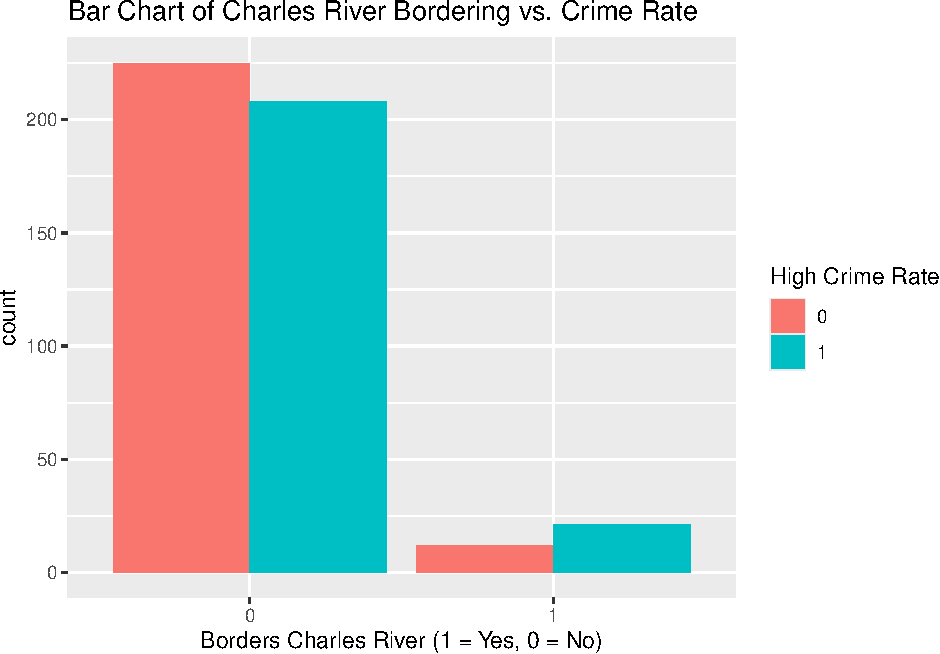
\includegraphics{Data-621-Hw4-Wa_files/figure-latex/unnamed-chunk-3-2.pdf}

\begin{Shaded}
\begin{Highlighting}[]
\CommentTok{\#  Check to see if relation ship are linear }


\CommentTok{\# relationship with Target flap}
\CommentTok{\# Boxplot of AGE by TARGET\_FLAG}
\FunctionTok{ggplot}\NormalTok{(training\_data, }\FunctionTok{aes}\NormalTok{(}\AttributeTok{x =} \FunctionTok{as.factor}\NormalTok{(TARGET\_FLAG), }\AttributeTok{y =}\NormalTok{ AGE)) }\SpecialCharTok{+}
  \FunctionTok{geom\_boxplot}\NormalTok{(}\AttributeTok{fill =} \StringTok{"purple"}\NormalTok{, }\AttributeTok{alpha =} \FloatTok{0.7}\NormalTok{) }\SpecialCharTok{+}
  \FunctionTok{labs}\NormalTok{(}\AttributeTok{title =} \StringTok{"Boxplot of AGE by TARGET\_FLAG"}\NormalTok{, }\AttributeTok{x =} \StringTok{"Crash (1) / No Crash (0)"}\NormalTok{, }\AttributeTok{y =} \StringTok{"Age"}\NormalTok{)}
\end{Highlighting}
\end{Shaded}

\includegraphics{Data-621-Hw4-Wa_files/figure-latex/unnamed-chunk-3-3.pdf}

\begin{Shaded}
\begin{Highlighting}[]
\CommentTok{\# Categorical variable distribution by TARGET\_FLAG}
\FunctionTok{ggplot}\NormalTok{(training\_data, }\FunctionTok{aes}\NormalTok{(}\AttributeTok{x =}\NormalTok{ CAR\_TYPE, }\AttributeTok{fill =} \FunctionTok{as.factor}\NormalTok{(TARGET\_FLAG))) }\SpecialCharTok{+}
  \FunctionTok{geom\_bar}\NormalTok{(}\AttributeTok{position =} \StringTok{"dodge"}\NormalTok{) }\SpecialCharTok{+}
  \FunctionTok{labs}\NormalTok{(}\AttributeTok{title =} \StringTok{"Car Type by TARGET\_FLAG"}\NormalTok{, }\AttributeTok{x =} \StringTok{"Car Type"}\NormalTok{, }\AttributeTok{y =} \StringTok{"Count"}\NormalTok{, }\AttributeTok{fill =} \StringTok{"Crash (1)/No Crash (0)"}\NormalTok{)}
\end{Highlighting}
\end{Shaded}

\includegraphics{Data-621-Hw4-Wa_files/figure-latex/unnamed-chunk-3-4.pdf}

\begin{Shaded}
\begin{Highlighting}[]
\FunctionTok{library}\NormalTok{(popbio)}
\end{Highlighting}
\end{Shaded}

\begin{verbatim}
## 
## Attaching package: 'popbio'
\end{verbatim}

\begin{verbatim}
## The following object is masked from 'package:caret':
## 
##     sensitivity
\end{verbatim}

\begin{Shaded}
\begin{Highlighting}[]
\NormalTok{numeric\_vars }\OtherTok{\textless{}{-}}\NormalTok{ numeric\_vars }\SpecialCharTok{\%\textgreater{}\%} \FunctionTok{mutate}\NormalTok{(}\FunctionTok{across}\NormalTok{(}\FunctionTok{where}\NormalTok{(is.character), }\SpecialCharTok{\textasciitilde{}} \FunctionTok{suppressWarnings}\NormalTok{(}\FunctionTok{as.numeric}\NormalTok{(.))))}
\NormalTok{x }\OtherTok{\textless{}{-}}\NormalTok{ training\_data[,]}
\NormalTok{x }\OtherTok{\textless{}{-}}\NormalTok{ x[}\SpecialCharTok{!}\FunctionTok{is.na}\NormalTok{(x}\SpecialCharTok{$}\NormalTok{AGE) }\SpecialCharTok{\&} \FunctionTok{is.finite}\NormalTok{(x}\SpecialCharTok{$}\NormalTok{AGE), ]}
\NormalTok{x}\SpecialCharTok{$}\NormalTok{AGE }\OtherTok{\textless{}{-}} \FunctionTok{as.numeric}\NormalTok{(}\FunctionTok{as.character}\NormalTok{(x}\SpecialCharTok{$}\NormalTok{AGE))}
\NormalTok{x}\SpecialCharTok{$}\NormalTok{YOJ }\OtherTok{\textless{}{-}} \FunctionTok{as.numeric}\NormalTok{(}\FunctionTok{as.character}\NormalTok{(x}\SpecialCharTok{$}\NormalTok{YOJ))}
\NormalTok{x}\SpecialCharTok{$}\NormalTok{CAR\_AGE }\OtherTok{\textless{}{-}} \FunctionTok{as.numeric}\NormalTok{(}\FunctionTok{as.character}\NormalTok{(x}\SpecialCharTok{$}\NormalTok{CAR\_AGE))}


\FunctionTok{par}\NormalTok{(}\AttributeTok{mfrow=}\FunctionTok{c}\NormalTok{(}\DecValTok{3}\NormalTok{,}\DecValTok{3}\NormalTok{))}
\FunctionTok{logi.hist.plot}\NormalTok{(x}\SpecialCharTok{$}\NormalTok{KIDSDRIV,x}\SpecialCharTok{$}\NormalTok{TARGET\_FLAG,}\AttributeTok{logi.mod =} \DecValTok{1}\NormalTok{, }\AttributeTok{type=}\StringTok{"p"}\NormalTok{, }\AttributeTok{boxp=}\ConstantTok{FALSE}\NormalTok{,}\AttributeTok{col=}\StringTok{"gray"}\NormalTok{, }\AttributeTok{mainlabel =} \StringTok{"Driving Children"}\NormalTok{)}

\FunctionTok{logi.hist.plot}\NormalTok{(x}\SpecialCharTok{$}\NormalTok{AGE, x}\SpecialCharTok{$}\NormalTok{TARGET\_FLAG,}\AttributeTok{logi.mod =} \DecValTok{1}\NormalTok{, }\AttributeTok{type=}\StringTok{"hist"}\NormalTok{,}\AttributeTok{boxp=}\ConstantTok{FALSE}\NormalTok{,}\AttributeTok{col=}\StringTok{"gray"}\NormalTok{, }\AttributeTok{mainlabel =} \StringTok{"Age of Driver"}\NormalTok{)}
\FunctionTok{logi.hist.plot}\NormalTok{(x}\SpecialCharTok{$}\NormalTok{HOMEKIDS,x}\SpecialCharTok{$}\NormalTok{TARGET\_FLAG,}\AttributeTok{logi.mod =} \DecValTok{1}\NormalTok{,}\AttributeTok{boxp=}\ConstantTok{FALSE}\NormalTok{,}\AttributeTok{type=}\StringTok{"hist"}\NormalTok{,}\AttributeTok{col=}\StringTok{"gray"}\NormalTok{, }\AttributeTok{mainlabel =} \StringTok{"Children at Home"}\NormalTok{)}
\NormalTok{x }\OtherTok{\textless{}{-}}\NormalTok{ x[}\SpecialCharTok{!}\FunctionTok{is.na}\NormalTok{(x}\SpecialCharTok{$}\NormalTok{YOJ) }\SpecialCharTok{\&} \FunctionTok{is.finite}\NormalTok{(x}\SpecialCharTok{$}\NormalTok{YOJ), ]}
\FunctionTok{logi.hist.plot}\NormalTok{(x}\SpecialCharTok{$}\NormalTok{YOJ, x}\SpecialCharTok{$}\NormalTok{TARGET\_FLAG,}\AttributeTok{logi.mod =} \DecValTok{1}\NormalTok{,}\AttributeTok{type=}\StringTok{"hist"}\NormalTok{,}\AttributeTok{boxp=}\ConstantTok{FALSE}\NormalTok{,}\AttributeTok{col=}\StringTok{"gray"}\NormalTok{, }\AttributeTok{mainlabel =} \StringTok{"Years on Job"}\NormalTok{)}
\CommentTok{\#logi.hist.plot(x$INCOME,x$TARGET\_FLAG,logi.mod = 1,boxp=FALSE,type="hist",col="gray", mainlabel = "rm")}
\FunctionTok{logi.hist.plot}\NormalTok{(x}\SpecialCharTok{$}\NormalTok{TRAVTIME       , x}\SpecialCharTok{$}\NormalTok{TARGET\_FLAG,}\AttributeTok{logi.mod =} \DecValTok{1}\NormalTok{,}\AttributeTok{type=}\StringTok{"hist"}\NormalTok{,}\AttributeTok{boxp=}\ConstantTok{FALSE}\NormalTok{,}\AttributeTok{col=}\StringTok{"gray"}\NormalTok{, }\AttributeTok{mainlabel =} \StringTok{"Distance to Work"}\NormalTok{)}
\CommentTok{\#logi.hist.plot(x$HOME\_VAL   ,x$TARGET\_FLAG,logi.mod = 1,boxp=FALSE,type="hist",col="gray", mainlabel = "dis")}
\CommentTok{\#logi.hist.plot(x$MSTATUS    , x$TARGET\_FLAG,logi.mod = 1,type="hist",boxp=FALSE,col="gray", mainlabel = "rad")}
\CommentTok{\#logi.hist.plot(x$SEX        ,x$TARGET\_FLAG,logi.mod = 1,boxp=FALSE,type="hist",col="gray", mainlabel = "tax")}
\CommentTok{\#logi.hist.plot(x$BLUEBOOK     , x$TARGET\_FLAG,logi.mod = 1,type="hist",boxp=FALSE,col="gray", mainlabel = "ptratio")}
\CommentTok{\#logi.hist.plot(x$black,x$TARGET\_FLAG,logi.mod = 1,boxp=FALSE,type="hist",col="gray", mainlabel = "black")}
\FunctionTok{logi.hist.plot}\NormalTok{(x}\SpecialCharTok{$}\NormalTok{TIF, x}\SpecialCharTok{$}\NormalTok{TARGET\_FLAG,}\AttributeTok{logi.mod =} \DecValTok{1}\NormalTok{,}\AttributeTok{type=}\StringTok{"hist"}\NormalTok{,}\AttributeTok{boxp=}\ConstantTok{FALSE}\NormalTok{,}\AttributeTok{col=}\StringTok{"gray"}\NormalTok{, }\AttributeTok{mainlabel =} \StringTok{"Time in Force"}\NormalTok{)}
\CommentTok{\#logi.hist.plot(x$RED\_CAR , x$TARGET\_FLAG,logi.mod = 1,type="hist",boxp=FALSE,col="gray", mainlabel = "medv")}
\CommentTok{\#logi.hist.plot(x$OLDCLAIM, x$TARGET\_FLAG,logi.mod = 1,type="hist",boxp=FALSE,col="gray", mainlabel = "lstat")}
\FunctionTok{logi.hist.plot}\NormalTok{(x}\SpecialCharTok{$}\NormalTok{CLM\_FREQ, x}\SpecialCharTok{$}\NormalTok{TARGET\_FLAG,}\AttributeTok{logi.mod =} \DecValTok{1}\NormalTok{,}\AttributeTok{type=}\StringTok{"hist"}\NormalTok{,}\AttributeTok{boxp=}\ConstantTok{FALSE}\NormalTok{,}\AttributeTok{col=}\StringTok{"gray"}\NormalTok{, }\AttributeTok{mainlabel =} \StringTok{"Claims (Past 5 Years)"}\NormalTok{)}
\CommentTok{\#logi.hist.plot(x$REVOKED, x$TARGET\_FLAG,logi.mod = 1,type="hist",boxp=FALSE,col="gray", mainlabel = "lstat")}
\CommentTok{\#logi.hist.plot(x$VR\_PTS, x$TARGET\_FLAG,logi.mod = 1,type="hist",boxp=FALSE,col="gray", mainlabel = "lstat")}
\NormalTok{x }\OtherTok{\textless{}{-}}\NormalTok{ x[}\SpecialCharTok{!}\FunctionTok{is.na}\NormalTok{(x}\SpecialCharTok{$}\NormalTok{CAR\_AGE) }\SpecialCharTok{\&} \FunctionTok{is.finite}\NormalTok{(x}\SpecialCharTok{$}\NormalTok{CAR\_AGE), ]}
\FunctionTok{logi.hist.plot}\NormalTok{(x}\SpecialCharTok{$}\NormalTok{CAR\_AGE, x}\SpecialCharTok{$}\NormalTok{TARGET\_FLAG,}\AttributeTok{logi.mod =} \DecValTok{1}\NormalTok{,}\AttributeTok{type=}\StringTok{"hist"}\NormalTok{,}\AttributeTok{boxp=}\ConstantTok{FALSE}\NormalTok{,}\AttributeTok{col=}\StringTok{"gray"}\NormalTok{, }\AttributeTok{mainlabel =} \StringTok{"Vehicle Age"}\NormalTok{)}
\end{Highlighting}
\end{Shaded}

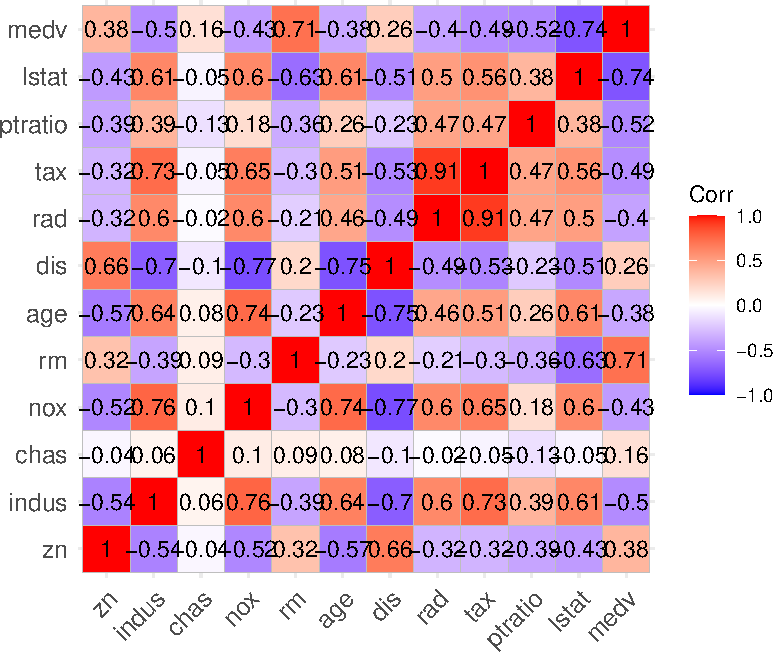
\includegraphics{Data-621-Hw4-Wa_files/figure-latex/unnamed-chunk-4-1.pdf}

\section{Conversion of Categoricall values to Numerical
Values}\label{conversion-of-categoricall-values-to-numerical-values}

The data has 8161 observations and 25 variables (excluding the
\texttt{INDEX} which won't be used for the analysis).

The primary target variable is \texttt{TARGET\_FLAG}, a binary indicator
representing whether a car was in crash, and the secondary target
\texttt{TARGET\_AMT} indicates the amount of the cost if a car was in
crash.

\texttt{AGE} has a mean of 44.8 years (SD = 14.3) with a median age of
45, indicating a balanced age distribution. \texttt{TRAVTIME} (commute
time to work) averages 33.5 minutes, with most values clustered between
22 and 44 minutes. A full table of key statistics is included above for
reference.

Several variables have missing values:

\begin{itemize}
\item
  \texttt{AGE} (6 missing values), \texttt{YOJ} (454), \texttt{INCOME}
  (many blanks), and \texttt{CAR\_AGE} (510). We are going to apply
  imputation strategies to address these gaps. Missing AGE values will
  be replaced with the median (45 years).
\item
  \texttt{YOJ} and \texttt{CAR\_AGE} will be imputed using their median
  values (11 and 8 years, respectively). \texttt{INCOME}, recorded as
  character strings, will be cleaned and converted to numeric, with
  missing values replaced by the median.
\end{itemize}

\begin{Shaded}
\begin{Highlighting}[]
\CommentTok{\# Convert columns with dollar signs to numeric}
\NormalTok{convert\_to\_numeric }\OtherTok{\textless{}{-}} \ControlFlowTok{function}\NormalTok{(column) \{}
  \FunctionTok{as.numeric}\NormalTok{(}\FunctionTok{gsub}\NormalTok{(}\StringTok{"[$,]"}\NormalTok{, }\StringTok{""}\NormalTok{, column))}
\NormalTok{\}}

\NormalTok{training\_data}\SpecialCharTok{$}\NormalTok{INCOME }\OtherTok{\textless{}{-}} \FunctionTok{convert\_to\_numeric}\NormalTok{(training\_data}\SpecialCharTok{$}\NormalTok{INCOME)}
\NormalTok{training\_data}\SpecialCharTok{$}\NormalTok{HOME\_VAL }\OtherTok{\textless{}{-}} \FunctionTok{convert\_to\_numeric}\NormalTok{(training\_data}\SpecialCharTok{$}\NormalTok{HOME\_VAL)}
\NormalTok{training\_data}\SpecialCharTok{$}\NormalTok{BLUEBOOK }\OtherTok{\textless{}{-}} \FunctionTok{convert\_to\_numeric}\NormalTok{(training\_data}\SpecialCharTok{$}\NormalTok{BLUEBOOK)}
\NormalTok{training\_data}\SpecialCharTok{$}\NormalTok{OLDCLAIM }\OtherTok{\textless{}{-}} \FunctionTok{convert\_to\_numeric}\NormalTok{(training\_data}\SpecialCharTok{$}\NormalTok{OLDCLAIM)}

\NormalTok{training\_data}\SpecialCharTok{$}\NormalTok{INCOME[}\FunctionTok{is.na}\NormalTok{(training\_data}\SpecialCharTok{$}\NormalTok{INCOME)] }\OtherTok{\textless{}{-}} \FunctionTok{median}\NormalTok{(training\_data}\SpecialCharTok{$}\NormalTok{INCOME, }\AttributeTok{na.rm =} \ConstantTok{TRUE}\NormalTok{)}
\NormalTok{training\_data}\SpecialCharTok{$}\NormalTok{HOME\_VAL[}\FunctionTok{is.na}\NormalTok{(training\_data}\SpecialCharTok{$}\NormalTok{HOME\_VAL)] }\OtherTok{\textless{}{-}} \FunctionTok{median}\NormalTok{(training\_data}\SpecialCharTok{$}\NormalTok{HOME\_VAL, }\AttributeTok{na.rm =} \ConstantTok{TRUE}\NormalTok{)}
\NormalTok{training\_data}\SpecialCharTok{$}\NormalTok{BLUEBOOK[}\FunctionTok{is.na}\NormalTok{(training\_data}\SpecialCharTok{$}\NormalTok{BLUEBOOK)] }\OtherTok{\textless{}{-}} \FunctionTok{median}\NormalTok{(training\_data}\SpecialCharTok{$}\NormalTok{BLUEBOOK, }\AttributeTok{na.rm =} \ConstantTok{TRUE}\NormalTok{)}
\NormalTok{training\_data}\SpecialCharTok{$}\NormalTok{OLDCLAIM[}\FunctionTok{is.na}\NormalTok{(training\_data}\SpecialCharTok{$}\NormalTok{OLDCLAIM)] }\OtherTok{\textless{}{-}} \FunctionTok{median}\NormalTok{(training\_data}\SpecialCharTok{$}\NormalTok{OLDCLAIM, }\AttributeTok{na.rm =} \ConstantTok{TRUE}\NormalTok{)}

\DocumentationTok{\#\#\# See the categorical Values }
\FunctionTok{table}\NormalTok{(training\_data}\SpecialCharTok{$}\NormalTok{PARENT1)}
\end{Highlighting}
\end{Shaded}

\begin{verbatim}
## 
##   No  Yes 
## 7084 1077
\end{verbatim}

\begin{Shaded}
\begin{Highlighting}[]
\FunctionTok{table}\NormalTok{(training\_data}\SpecialCharTok{$}\NormalTok{MSTATUS)}
\end{Highlighting}
\end{Shaded}

\begin{verbatim}
## 
##  Yes z_No 
## 4894 3267
\end{verbatim}

\begin{Shaded}
\begin{Highlighting}[]
\FunctionTok{table}\NormalTok{(training\_data}\SpecialCharTok{$}\NormalTok{URBANICITY)}
\end{Highlighting}
\end{Shaded}

\begin{verbatim}
## 
##   Highly Urban/ Urban z_Highly Rural/ Rural 
##                  6492                  1669
\end{verbatim}

\begin{Shaded}
\begin{Highlighting}[]
\FunctionTok{table}\NormalTok{(training\_data}\SpecialCharTok{$}\NormalTok{REVOKED )}
\end{Highlighting}
\end{Shaded}

\begin{verbatim}
## 
##   No  Yes 
## 7161 1000
\end{verbatim}

\begin{Shaded}
\begin{Highlighting}[]
\FunctionTok{table}\NormalTok{(training\_data}\SpecialCharTok{$}\NormalTok{RED\_CAR)}
\end{Highlighting}
\end{Shaded}

\begin{verbatim}
## 
##   no  yes 
## 5783 2378
\end{verbatim}

\begin{Shaded}
\begin{Highlighting}[]
\FunctionTok{table}\NormalTok{(training\_data}\SpecialCharTok{$}\NormalTok{SEX)}
\end{Highlighting}
\end{Shaded}

\begin{verbatim}
## 
##    M  z_F 
## 3786 4375
\end{verbatim}

\begin{Shaded}
\begin{Highlighting}[]
\FunctionTok{table}\NormalTok{(training\_data}\SpecialCharTok{$}\NormalTok{CAR\_TYPE)}\CommentTok{\# require more work}
\end{Highlighting}
\end{Shaded}

\begin{verbatim}
## 
##     Minivan Panel Truck      Pickup  Sports Car         Van       z_SUV 
##        2145         676        1389         907         750        2294
\end{verbatim}

\begin{Shaded}
\begin{Highlighting}[]
\FunctionTok{table}\NormalTok{(training\_data}\SpecialCharTok{$}\NormalTok{CAR\_USE)}
\end{Highlighting}
\end{Shaded}

\begin{verbatim}
## 
## Commercial    Private 
##       3029       5132
\end{verbatim}

\begin{Shaded}
\begin{Highlighting}[]
\FunctionTok{table}\NormalTok{(training\_data}\SpecialCharTok{$}\NormalTok{EDUCATION)}
\end{Highlighting}
\end{Shaded}

\begin{verbatim}
## 
##  <High School     Bachelors       Masters           PhD z_High School 
##          1203          2242          1658           728          2330
\end{verbatim}

\begin{Shaded}
\begin{Highlighting}[]
\CommentTok{\# Convert categorical variable }
\NormalTok{training\_data}\SpecialCharTok{$}\NormalTok{PARENT1 }\OtherTok{\textless{}{-}} \FunctionTok{ifelse}\NormalTok{(training\_data}\SpecialCharTok{$}\NormalTok{PARENT1 }\SpecialCharTok{==} \StringTok{"Yes"}\NormalTok{, }\DecValTok{1}\NormalTok{, }\DecValTok{0}\NormalTok{) }\CommentTok{\# 1 for Yes and 0 for No}
\NormalTok{training\_data}\SpecialCharTok{$}\NormalTok{MSTATUS }\OtherTok{\textless{}{-}} \FunctionTok{ifelse}\NormalTok{(training\_data}\SpecialCharTok{$}\NormalTok{MSTATUS }\SpecialCharTok{==} \StringTok{"Yes"}\NormalTok{, }\DecValTok{1}\NormalTok{, }\DecValTok{0}\NormalTok{) }\CommentTok{\# 1 for Yes and 0 z\_NO}
\NormalTok{training\_data}\SpecialCharTok{$}\NormalTok{URBANICITY }\OtherTok{\textless{}{-}} \FunctionTok{ifelse}\NormalTok{(training\_data}\SpecialCharTok{$}\NormalTok{URBANICITY }\SpecialCharTok{==} \StringTok{"Highly Urban/ Urban"}\NormalTok{, }\DecValTok{1}\NormalTok{, }\DecValTok{0}\NormalTok{) }\DocumentationTok{\#\#\#\# Highly Urban/ Urban 1 and 0 z\_Highly Rural/ Rural}
\NormalTok{training\_data}\SpecialCharTok{$}\NormalTok{REVOKED  }\OtherTok{\textless{}{-}} \FunctionTok{ifelse}\NormalTok{(training\_data}\SpecialCharTok{$}\NormalTok{REVOKED  }\SpecialCharTok{==} \StringTok{"Yes"}\NormalTok{, }\DecValTok{1}\NormalTok{, }\DecValTok{0}\NormalTok{) }\CommentTok{\# 1 for Yes and 0 for No}
\NormalTok{training\_data}\SpecialCharTok{$}\NormalTok{RED\_CAR }\OtherTok{\textless{}{-}} \FunctionTok{ifelse}\NormalTok{(training\_data}\SpecialCharTok{$}\NormalTok{RED\_CAR }\SpecialCharTok{==} \StringTok{"yes"}\NormalTok{, }\DecValTok{1}\NormalTok{, }\DecValTok{0}\NormalTok{) }\CommentTok{\# 1 for Yes and 0 for No}
\NormalTok{training\_data}\SpecialCharTok{$}\NormalTok{SEX  }\OtherTok{\textless{}{-}} \FunctionTok{ifelse}\NormalTok{(training\_data}\SpecialCharTok{$}\NormalTok{SEX  }\SpecialCharTok{==} \StringTok{"M"}\NormalTok{, }\DecValTok{1}\NormalTok{, }\DecValTok{0}\NormalTok{) }\CommentTok{\# 1 for M and 0 for z\_F}
\NormalTok{training\_data}\SpecialCharTok{$}\NormalTok{CAR\_USE }\OtherTok{\textless{}{-}} \FunctionTok{ifelse}\NormalTok{(training\_data}\SpecialCharTok{$}\NormalTok{CAR\_USE }\SpecialCharTok{==} \StringTok{"Private"}\NormalTok{, }\DecValTok{1}\NormalTok{, }\DecValTok{0}\NormalTok{)  }\CommentTok{\# 1 for Private and 0 for Commercial }

\CommentTok{\# Convert CAR\_TYPE to a factor and then to numeric}
\NormalTok{training\_data}\SpecialCharTok{$}\NormalTok{CAR\_TYPE }\OtherTok{\textless{}{-}} \FunctionTok{as.numeric}\NormalTok{(}\FunctionTok{as.factor}\NormalTok{(training\_data}\SpecialCharTok{$}\NormalTok{CAR\_TYPE))}
\CommentTok{\# Check the mapping of levels to numbers}
\FunctionTok{levels}\NormalTok{(}\FunctionTok{as.factor}\NormalTok{(training\_data}\SpecialCharTok{$}\NormalTok{CAR\_TYPE)) }\CommentTok{\# \# Convert CAR\_TYPE to a factor and then to numeric }
\end{Highlighting}
\end{Shaded}

\begin{verbatim}
## [1] "1" "2" "3" "4" "5" "6"
\end{verbatim}

\begin{Shaded}
\begin{Highlighting}[]
\CommentTok{\# Minivan Panel = 1 Truck =2      Pickup= 3  Sports Car = 4        Van = 5      z\_SUV = 6}


\CommentTok{\# Convert EDUCATION to a factor and then to numeric}
\NormalTok{training\_data}\SpecialCharTok{$}\NormalTok{EDUCATION }\OtherTok{\textless{}{-}} \FunctionTok{as.numeric}\NormalTok{(}\FunctionTok{as.factor}\NormalTok{(training\_data}\SpecialCharTok{$}\NormalTok{EDUCATION))}
\CommentTok{\# Check the mapping of levels to numbers}
\FunctionTok{levels}\NormalTok{(}\FunctionTok{as.factor}\NormalTok{(training\_data}\SpecialCharTok{$}\NormalTok{EDUCATION)) }
\end{Highlighting}
\end{Shaded}

\begin{verbatim}
## [1] "1" "2" "3" "4" "5"
\end{verbatim}

\begin{Shaded}
\begin{Highlighting}[]
\FunctionTok{summary}\NormalTok{(training\_data)}
\end{Highlighting}
\end{Shaded}

\begin{verbatim}
##      INDEX        TARGET_FLAG       TARGET_AMT        KIDSDRIV     
##  Min.   :    1   Min.   :0.0000   Min.   :     0   Min.   :0.0000  
##  1st Qu.: 2559   1st Qu.:0.0000   1st Qu.:     0   1st Qu.:0.0000  
##  Median : 5133   Median :0.0000   Median :     0   Median :0.0000  
##  Mean   : 5152   Mean   :0.2638   Mean   :  1504   Mean   :0.1711  
##  3rd Qu.: 7745   3rd Qu.:1.0000   3rd Qu.:  1036   3rd Qu.:0.0000  
##  Max.   :10302   Max.   :1.0000   Max.   :107586   Max.   :4.0000  
##                                                                    
##       AGE           HOMEKIDS           YOJ           INCOME      
##  Min.   :16.00   Min.   :0.0000   Min.   : 0.0   Min.   :     0  
##  1st Qu.:39.00   1st Qu.:0.0000   1st Qu.: 9.0   1st Qu.: 29707  
##  Median :45.00   Median :0.0000   Median :11.0   Median : 54028  
##  Mean   :44.79   Mean   :0.7212   Mean   :10.5   Mean   : 61469  
##  3rd Qu.:51.00   3rd Qu.:1.0000   3rd Qu.:13.0   3rd Qu.: 83304  
##  Max.   :81.00   Max.   :5.0000   Max.   :23.0   Max.   :367030  
##  NA's   :6                        NA's   :454                    
##     PARENT1         HOME_VAL         MSTATUS            SEX        
##  Min.   :0.000   Min.   :     0   Min.   :0.0000   Min.   :0.0000  
##  1st Qu.:0.000   1st Qu.:     0   1st Qu.:0.0000   1st Qu.:0.0000  
##  Median :0.000   Median :161160   Median :1.0000   Median :0.0000  
##  Mean   :0.132   Mean   :155225   Mean   :0.5997   Mean   :0.4639  
##  3rd Qu.:0.000   3rd Qu.:233352   3rd Qu.:1.0000   3rd Qu.:1.0000  
##  Max.   :1.000   Max.   :885282   Max.   :1.0000   Max.   :1.0000  
##                                                                    
##    EDUCATION         JOB               TRAVTIME         CAR_USE      
##  Min.   :1.000   Length:8161        Min.   :  5.00   Min.   :0.0000  
##  1st Qu.:2.000   Class :character   1st Qu.: 22.00   1st Qu.:0.0000  
##  Median :3.000   Mode  :character   Median : 33.00   Median :1.0000  
##  Mean   :3.091                      Mean   : 33.49   Mean   :0.6288  
##  3rd Qu.:5.000                      3rd Qu.: 44.00   3rd Qu.:1.0000  
##  Max.   :5.000                      Max.   :142.00   Max.   :1.0000  
##                                                                      
##     BLUEBOOK          TIF            CAR_TYPE       RED_CAR      
##  Min.   : 1500   Min.   : 1.000   Min.   :1.00   Min.   :0.0000  
##  1st Qu.: 9280   1st Qu.: 1.000   1st Qu.:1.00   1st Qu.:0.0000  
##  Median :14440   Median : 4.000   Median :3.00   Median :0.0000  
##  Mean   :15710   Mean   : 5.351   Mean   :3.53   Mean   :0.2914  
##  3rd Qu.:20850   3rd Qu.: 7.000   3rd Qu.:6.00   3rd Qu.:1.0000  
##  Max.   :69740   Max.   :25.000   Max.   :6.00   Max.   :1.0000  
##                                                                  
##     OLDCLAIM        CLM_FREQ         REVOKED          MVR_PTS      
##  Min.   :    0   Min.   :0.0000   Min.   :0.0000   Min.   : 0.000  
##  1st Qu.:    0   1st Qu.:0.0000   1st Qu.:0.0000   1st Qu.: 0.000  
##  Median :    0   Median :0.0000   Median :0.0000   Median : 1.000  
##  Mean   : 4037   Mean   :0.7986   Mean   :0.1225   Mean   : 1.696  
##  3rd Qu.: 4636   3rd Qu.:2.0000   3rd Qu.:0.0000   3rd Qu.: 3.000  
##  Max.   :57037   Max.   :5.0000   Max.   :1.0000   Max.   :13.000  
##                                                                    
##     CAR_AGE         URBANICITY    
##  Min.   :-3.000   Min.   :0.0000  
##  1st Qu.: 1.000   1st Qu.:1.0000  
##  Median : 8.000   Median :1.0000  
##  Mean   : 8.328   Mean   :0.7955  
##  3rd Qu.:12.000   3rd Qu.:1.0000  
##  Max.   :28.000   Max.   :1.0000  
##  NA's   :510
\end{verbatim}

\subsubsection{b. Creating Flags for Missing
Values:}\label{b.-creating-flags-for-missing-values}

\begin{Shaded}
\begin{Highlighting}[]
\NormalTok{insurance\_training }\OtherTok{\textless{}{-}}\NormalTok{ training\_data}
\CommentTok{\# Loop through all variables to create flags for missing values}
\ControlFlowTok{for}\NormalTok{ (var }\ControlFlowTok{in} \FunctionTok{colnames}\NormalTok{(insurance\_training)) \{}
\NormalTok{  insurance\_training[}\FunctionTok{paste0}\NormalTok{(var, }\StringTok{"\_FLAG"}\NormalTok{)] }\OtherTok{\textless{}{-}} \FunctionTok{ifelse}\NormalTok{(}\FunctionTok{is.na}\NormalTok{(insurance\_training[[var]]), }\DecValTok{1}\NormalTok{, }\DecValTok{0}\NormalTok{)}
\NormalTok{\}}

\CommentTok{\# Check the new flags columns}
\FunctionTok{head}\NormalTok{(insurance\_training)}
\end{Highlighting}
\end{Shaded}

\begin{verbatim}
##   INDEX TARGET_FLAG TARGET_AMT KIDSDRIV AGE HOMEKIDS YOJ INCOME PARENT1
## 1     1           0          0        0  60        0  11  67349       0
## 2     2           0          0        0  43        0  11  91449       0
## 3     4           0          0        0  35        1  10  16039       0
## 4     5           0          0        0  51        0  14  54028       0
## 5     6           0          0        0  50        0  NA 114986       0
## 6     7           1       2946        0  34        1  12 125301       1
##   HOME_VAL MSTATUS SEX EDUCATION           JOB TRAVTIME CAR_USE BLUEBOOK TIF
## 1        0       0   1         4  Professional       14       1    14230  11
## 2   257252       0   1         5 z_Blue Collar       22       0    14940   1
## 3   124191       1   0         5      Clerical        5       1     4010   4
## 4   306251       1   1         1 z_Blue Collar       32       1    15440   7
## 5   243925       1   0         4        Doctor       36       1    18000   1
## 6        0       0   0         2 z_Blue Collar       46       0    17430   1
##   CAR_TYPE RED_CAR OLDCLAIM CLM_FREQ REVOKED MVR_PTS CAR_AGE URBANICITY
## 1        1       1     4461        2       0       3      18          1
## 2        1       1        0        0       0       0       1          1
## 3        6       0    38690        2       0       3      10          1
## 4        1       1        0        0       0       0       6          1
## 5        6       0    19217        2       1       3      17          1
## 6        4       0        0        0       0       0       7          1
##   INDEX_FLAG TARGET_FLAG_FLAG TARGET_AMT_FLAG KIDSDRIV_FLAG AGE_FLAG
## 1          0                0               0             0        0
## 2          0                0               0             0        0
## 3          0                0               0             0        0
## 4          0                0               0             0        0
## 5          0                0               0             0        0
## 6          0                0               0             0        0
##   HOMEKIDS_FLAG YOJ_FLAG INCOME_FLAG PARENT1_FLAG HOME_VAL_FLAG MSTATUS_FLAG
## 1             0        0           0            0             0            0
## 2             0        0           0            0             0            0
## 3             0        0           0            0             0            0
## 4             0        0           0            0             0            0
## 5             0        1           0            0             0            0
## 6             0        0           0            0             0            0
##   SEX_FLAG EDUCATION_FLAG JOB_FLAG TRAVTIME_FLAG CAR_USE_FLAG BLUEBOOK_FLAG
## 1        0              0        0             0            0             0
## 2        0              0        0             0            0             0
## 3        0              0        0             0            0             0
## 4        0              0        0             0            0             0
## 5        0              0        0             0            0             0
## 6        0              0        0             0            0             0
##   TIF_FLAG CAR_TYPE_FLAG RED_CAR_FLAG OLDCLAIM_FLAG CLM_FREQ_FLAG REVOKED_FLAG
## 1        0             0            0             0             0            0
## 2        0             0            0             0             0            0
## 3        0             0            0             0             0            0
## 4        0             0            0             0             0            0
## 5        0             0            0             0             0            0
## 6        0             0            0             0             0            0
##   MVR_PTS_FLAG CAR_AGE_FLAG URBANICITY_FLAG
## 1            0            0               0
## 2            0            0               0
## 3            0            0               0
## 4            0            0               0
## 5            0            0               0
## 6            0            0               0
\end{verbatim}

\begin{itemize}
\item
  The paste0(var, ``\_FLAG'') dynamically creates the name for the new
  flag column based on the original variable name (e.g., if the original
  variable is AGE, the flag column will be AGE\_FLAG).
\item
  ifelse(is.na(insurance\_training{[}{[}var{]}{]}), 1, 0) checks if the
  value is missing (NA), and if it is, it assigns a 1; otherwise, it
  assigns a 0.
\end{itemize}

\subsubsection{c.~Transforming data by putting it into
buckets:}\label{c.-transforming-data-by-putting-it-into-buckets}

In this sub-section, we are going to bucketize the continuous variables;
\texttt{AGE} and \texttt{TARGET\_AMT}:

\begin{Shaded}
\begin{Highlighting}[]
\CommentTok{\# Bucketize AGE into ranges}
\NormalTok{insurance\_training}\SpecialCharTok{$}\NormalTok{AGE\_BUCKET }\OtherTok{\textless{}{-}} \FunctionTok{cut}\NormalTok{(insurance\_training}\SpecialCharTok{$}\NormalTok{AGE,}
                                \AttributeTok{breaks =} \FunctionTok{c}\NormalTok{(}\DecValTok{18}\NormalTok{, }\DecValTok{30}\NormalTok{, }\DecValTok{50}\NormalTok{, }\DecValTok{70}\NormalTok{, }\ConstantTok{Inf}\NormalTok{),}
                                \AttributeTok{labels =} \FunctionTok{c}\NormalTok{(}\StringTok{"18{-}30"}\NormalTok{, }\StringTok{"31{-}50"}\NormalTok{, }\StringTok{"51{-}70"}\NormalTok{, }\StringTok{"70+"}\NormalTok{))}

\CommentTok{\# Bucketize TARGET\_AMT into categories}
\NormalTok{insurance\_training}\SpecialCharTok{$}\NormalTok{TARGET\_AMT\_BUCKET }\OtherTok{\textless{}{-}} \FunctionTok{cut}\NormalTok{(insurance\_training}\SpecialCharTok{$}\NormalTok{TARGET\_AMT,}
                                       \AttributeTok{breaks =} \FunctionTok{c}\NormalTok{(}\DecValTok{0}\NormalTok{, }\DecValTok{1000}\NormalTok{, }\DecValTok{5000}\NormalTok{, }\DecValTok{10000}\NormalTok{, }\ConstantTok{Inf}\NormalTok{),}
                                       \AttributeTok{labels =} \FunctionTok{c}\NormalTok{(}\StringTok{"0{-}1000"}\NormalTok{, }\StringTok{"1001{-}5000"}\NormalTok{, }\StringTok{"5001{-}10000"}\NormalTok{, }\StringTok{"10000+"}\NormalTok{))}

\CommentTok{\# Check the bucketized varaibles}
\FunctionTok{table}\NormalTok{(insurance\_training}\SpecialCharTok{$}\NormalTok{AGE\_BUCKET)}
\end{Highlighting}
\end{Shaded}

\begin{verbatim}
## 
## 18-30 31-50 51-70   70+ 
##   400  5632  2105     9
\end{verbatim}

\begin{Shaded}
\begin{Highlighting}[]
\FunctionTok{table}\NormalTok{(insurance\_training}\SpecialCharTok{$}\NormalTok{TARGET\_AMT\_BUCKET)}
\end{Highlighting}
\end{Shaded}

\begin{verbatim}
## 
##     0-1000  1001-5000 5001-10000     10000+ 
##        102       1267        629        155
\end{verbatim}

By bucketizing \texttt{AGE} into discrete categories, it makes the
variable easier to interpret and analyze. Similarly, bucketizing
\texttt{TARGET\_AMT} helps transform a continuous variable with
potentially high variation into manageable categories. This can help
with clearer reporting and analysis of trends.

\subsubsection{d.~Mathematical transforms such as log or square root (or
use
Box-Cox):}\label{d.-mathematical-transforms-such-as-log-or-square-root-or-use-box-cox}

First and to have a clear decision about the type of transformation
based on the skewness of each variable:

\begin{Shaded}
\begin{Highlighting}[]
\FunctionTok{library}\NormalTok{(moments)}
\end{Highlighting}
\end{Shaded}

\begin{verbatim}
## 
## Attaching package: 'moments'
\end{verbatim}

\begin{verbatim}
## The following objects are masked from 'package:e1071':
## 
##     kurtosis, moment, skewness
\end{verbatim}

\begin{Shaded}
\begin{Highlighting}[]
\CommentTok{\# Check skewness for numeric variables}
\NormalTok{skew\_values }\OtherTok{\textless{}{-}} \FunctionTok{sapply}\NormalTok{(insurance\_training[, }\FunctionTok{c}\NormalTok{(}\StringTok{"AGE"}\NormalTok{, }\StringTok{"CAR\_AGE"}\NormalTok{, }\StringTok{"TARGET\_AMT"}\NormalTok{, }\StringTok{"KIDSDRIV"}\NormalTok{, }\StringTok{"HOMEKIDS"}\NormalTok{)], skewness, }\AttributeTok{na.rm =} \ConstantTok{TRUE}\NormalTok{)}

\CommentTok{\# View skewness values}
\FunctionTok{print}\NormalTok{(skew\_values)}
\end{Highlighting}
\end{Shaded}

\begin{verbatim}
##         AGE     CAR_AGE  TARGET_AMT    KIDSDRIV    HOMEKIDS 
## -0.02899428  0.28200841  8.70790384  3.35245360  1.34137363
\end{verbatim}

Interpretations:

\begin{itemize}
\item
  \texttt{AGE}: -0.03 This value is close to 0, indicating that the AGE
  variable is approximately normally distributed. No transformation is
  needed.
\item
  \texttt{CAR\_AGE}: 0.29 The skewness of CAR\_AGE is slightly positive,
  but it is relatively close to 0, meaning it is only mildly skewed. We
  may not need a transformation for this variable, as the skewness is
  not severe.
\item
  \texttt{TARGET\_AMT}: 8.71 This is highly positively skewed, with a
  skewness greater than 1. This suggests that TARGET\_AMT has a long
  right tail, which is typical for monetary data. \textbf{A log
  transformation} would be helpful in normalizing this variable.
\item
  \texttt{KIDSDRIV}: 3.35 This has significant positive skewness, but
  it's not extreme. If you want to reduce the skewness, you could
  consider a log transformation, but it might not be absolutely
  necessary if the model can handle the skewness well.
\item
  \texttt{HOMEKIDS}: 1.34 This value also indicates mild positive
  skewness. Similar to CAR\_AGE, no transformation is strictly
  necessary, but a log transformation could slightly improve the
  distribution, especially if we are aiming for perfect normality.
\end{itemize}

Now, based on the skewness above, we only need to log-transform the
\texttt{TARGET\_AMT}, and the other two variables that have a slight
high skewness:

\begin{Shaded}
\begin{Highlighting}[]
\CommentTok{\# Apply log transformation to TARGET\_AMT amd the others}
\NormalTok{insurance\_training}\SpecialCharTok{$}\NormalTok{TARGET\_AMT\_LOG }\OtherTok{\textless{}{-}} \FunctionTok{log}\NormalTok{(insurance\_training}\SpecialCharTok{$}\NormalTok{TARGET\_AMT }\SpecialCharTok{+} \DecValTok{1}\NormalTok{)}

\NormalTok{insurance\_training}\SpecialCharTok{$}\NormalTok{KIDSDRIV\_LOG }\OtherTok{\textless{}{-}} \FunctionTok{log}\NormalTok{(insurance\_training}\SpecialCharTok{$}\NormalTok{KIDSDRIV }\SpecialCharTok{+} \DecValTok{1}\NormalTok{)}
\NormalTok{insurance\_training}\SpecialCharTok{$}\NormalTok{HOMEKIDS\_LOG }\OtherTok{\textless{}{-}} \FunctionTok{log}\NormalTok{(insurance\_training}\SpecialCharTok{$}\NormalTok{HOMEKIDS }\SpecialCharTok{+} \DecValTok{1}\NormalTok{)}
\end{Highlighting}
\end{Shaded}

Let's check the skewness values after the transformations we performed
above:

\begin{Shaded}
\begin{Highlighting}[]
\CommentTok{\# Check skewness after applying the transformations}
\NormalTok{skew\_values\_after\_transformation }\OtherTok{\textless{}{-}} \FunctionTok{sapply}\NormalTok{(insurance\_training[, }\FunctionTok{c}\NormalTok{(}\StringTok{"AGE"}\NormalTok{, }\StringTok{"CAR\_AGE"}\NormalTok{, }\StringTok{"TARGET\_AMT\_LOG"}\NormalTok{, }\StringTok{"KIDSDRIV\_LOG"}\NormalTok{, }\StringTok{"HOMEKIDS\_LOG"}\NormalTok{)], skewness, }\AttributeTok{na.rm =} \ConstantTok{TRUE}\NormalTok{)}

\CommentTok{\# View the skewness values after transformation}
\FunctionTok{print}\NormalTok{(skew\_values\_after\_transformation)}
\end{Highlighting}
\end{Shaded}

\begin{verbatim}
##            AGE        CAR_AGE TARGET_AMT_LOG   KIDSDRIV_LOG   HOMEKIDS_LOG 
##    -0.02899428     0.28200841     1.11539275     2.73431737     0.93273108
\end{verbatim}

That is good progress;

\begin{itemize}
\item
  The log transformation on \texttt{TARGET\_AMT} has reduced the
  skewness significantly, but it remains moderately skewed. This is
  typical for monetary variables. The transformation has improved the
  distribution but could still benefit from further adjustments.
\item
  The transformation on \texttt{KIDSDRIV} has reduced the skewness but
  it is still quite positive. This suggests that the log transformation
  helped, but the variable is still somewhat skewed. We should consider
  another transformation.
\item
  The log transformation on \texttt{HOMEKIDS} has reduced the skewness
  to a more acceptable level, bringing it closer to zero. This variable
  is now much more normally distributed and ready for modeling.
\end{itemize}

One additional tranformation that can help us normalize the continuous
variable \texttt{TARGET\_AMT}is Box-Cox Transformation

\begin{Shaded}
\begin{Highlighting}[]
\NormalTok{insurance\_training}\SpecialCharTok{$}\NormalTok{TARGET\_AMT\_SHIFTED }\OtherTok{\textless{}{-}}\NormalTok{ insurance\_training}\SpecialCharTok{$}\NormalTok{TARGET\_AMT }\SpecialCharTok{+} \DecValTok{1}
\NormalTok{boxcox\_result }\OtherTok{\textless{}{-}} \FunctionTok{boxcox}\NormalTok{(TARGET\_AMT\_SHIFTED }\SpecialCharTok{\textasciitilde{}} \DecValTok{1}\NormalTok{, }\AttributeTok{data =}\NormalTok{ insurance\_training)}
\end{Highlighting}
\end{Shaded}

\includegraphics{Data-621-Hw4-Wa_files/figure-latex/unnamed-chunk-11-1.pdf}

\begin{Shaded}
\begin{Highlighting}[]
\NormalTok{lambda }\OtherTok{\textless{}{-}}\NormalTok{ boxcox\_result}\SpecialCharTok{$}\NormalTok{x[}\FunctionTok{which.max}\NormalTok{(boxcox\_result}\SpecialCharTok{$}\NormalTok{y)]}
\NormalTok{insurance\_training}\SpecialCharTok{$}\NormalTok{TARGET\_AMT\_BOXCOX }\OtherTok{\textless{}{-}}\NormalTok{ (insurance\_training}\SpecialCharTok{$}\NormalTok{TARGET\_AMT\_SHIFTED}\SpecialCharTok{\^{}}\NormalTok{lambda }\SpecialCharTok{{-}} \DecValTok{1}\NormalTok{) }\SpecialCharTok{/}\NormalTok{ lambda}
\end{Highlighting}
\end{Shaded}

we can also perform the square root transformation:

\begin{Shaded}
\begin{Highlighting}[]
\NormalTok{insurance\_training}\SpecialCharTok{$}\NormalTok{TARGET\_AMT\_SQRT }\OtherTok{\textless{}{-}} \FunctionTok{sqrt}\NormalTok{(insurance\_training}\SpecialCharTok{$}\NormalTok{TARGET\_AMT)}
\end{Highlighting}
\end{Shaded}

Let's do the same thing for the variable \texttt{KIDSDRIV}:

First, Box-Cox:

\begin{Shaded}
\begin{Highlighting}[]
\NormalTok{insurance\_training}\SpecialCharTok{$}\NormalTok{KIDSDRIV\_BOXCOX }\OtherTok{\textless{}{-}}\NormalTok{ (insurance\_training}\SpecialCharTok{$}\NormalTok{KIDSDRIV }\SpecialCharTok{+} \DecValTok{1}\NormalTok{)}\SpecialCharTok{\^{}}\NormalTok{lambda }\SpecialCharTok{{-}} \DecValTok{1}
\end{Highlighting}
\end{Shaded}

Then, we can use Cube Root transformation:

\begin{Shaded}
\begin{Highlighting}[]
\NormalTok{insurance\_training}\SpecialCharTok{$}\NormalTok{KIDSDRIV\_CUBE }\OtherTok{\textless{}{-}} \FunctionTok{sign}\NormalTok{(insurance\_training}\SpecialCharTok{$}\NormalTok{KIDSDRIV) }\SpecialCharTok{*} \FunctionTok{abs}\NormalTok{(insurance\_training}\SpecialCharTok{$}\NormalTok{KIDSDRIV)}\SpecialCharTok{\^{}}\NormalTok{(}\DecValTok{1}\SpecialCharTok{/}\DecValTok{3}\NormalTok{)}
\end{Highlighting}
\end{Shaded}

Let's check once more for after-transformations-skewness

\begin{Shaded}
\begin{Highlighting}[]
\CommentTok{\# Check skewness after applying the transformations}
\NormalTok{skew\_values\_after\_transformation2 }\OtherTok{\textless{}{-}} \FunctionTok{sapply}\NormalTok{(insurance\_training[, }\FunctionTok{c}\NormalTok{(}\StringTok{"AGE"}\NormalTok{, }\StringTok{"CAR\_AGE"}\NormalTok{, }\StringTok{"TARGET\_AMT\_BOXCOX"}\NormalTok{, }\StringTok{"KIDSDRIV\_BOXCOX"}\NormalTok{, }\StringTok{"HOMEKIDS\_LOG"}\NormalTok{)], skewness, }\AttributeTok{na.rm =} \ConstantTok{TRUE}\NormalTok{)}

\CommentTok{\# View the skewness values after transformation}
\FunctionTok{print}\NormalTok{(skew\_values\_after\_transformation2)}
\end{Highlighting}
\end{Shaded}

\begin{verbatim}
##               AGE           CAR_AGE TARGET_AMT_BOXCOX   KIDSDRIV_BOXCOX 
##       -0.02899428        0.28200841        1.07302400       -2.60416012 
##      HOMEKIDS_LOG 
##        0.93273108
\end{verbatim}

\begin{Shaded}
\begin{Highlighting}[]
\CommentTok{\# Check skewness after applying the transformations}
\NormalTok{skew\_values\_after\_transformation3 }\OtherTok{\textless{}{-}} \FunctionTok{sapply}\NormalTok{(insurance\_training[, }\FunctionTok{c}\NormalTok{(}\StringTok{"AGE"}\NormalTok{, }\StringTok{"CAR\_AGE"}\NormalTok{, }\StringTok{"TARGET\_AMT\_SQRT"}\NormalTok{, }\StringTok{"KIDSDRIV\_CUBE"}\NormalTok{, }\StringTok{"HOMEKIDS\_LOG"}\NormalTok{)], skewness, }\AttributeTok{na.rm =} \ConstantTok{TRUE}\NormalTok{)}

\CommentTok{\# View the skewness values after transformation}
\FunctionTok{print}\NormalTok{(skew\_values\_after\_transformation3)}
\end{Highlighting}
\end{Shaded}

\begin{verbatim}
##             AGE         CAR_AGE TARGET_AMT_SQRT   KIDSDRIV_CUBE    HOMEKIDS_LOG 
##     -0.02899428      0.28200841      2.34921703      2.43572837      0.93273108
\end{verbatim}

Based on the transformations above:

\begin{itemize}
\tightlist
\item
  \texttt{TARGET\_AMT}: Box-Cox was more effective in reducing skewness
  compared to the square root or cube transformations. While for
  \texttt{KIDSDRIV}, Box-Cox made the variable more negatively skewed,
  whereas cube transformation made it more positively skewed. Neither
  transformation worked well. So we better keep the \_CUBE or find
  another approach for this variable.
\end{itemize}

\subsubsection{e. Creating New
Variables:}\label{e.-creating-new-variables}

Age-based Grouping (AGE\_GROUP): Age is a continuous variable, but for
the purposes of analysis and modeling, grouping it into categories
allows us to better understand trends in different age ranges. For
example, it might be valuable to compare the behavior of individuals in
their 20s versus those in their 50s when it comes to claims or risk.

\begin{Shaded}
\begin{Highlighting}[]
\CommentTok{\# Create age groups}
\NormalTok{insurance\_training}\SpecialCharTok{$}\NormalTok{AGE\_GROUP }\OtherTok{\textless{}{-}} \FunctionTok{cut}\NormalTok{(insurance\_training}\SpecialCharTok{$}\NormalTok{AGE, }
                               \AttributeTok{breaks =} \FunctionTok{c}\NormalTok{(}\DecValTok{18}\NormalTok{, }\DecValTok{30}\NormalTok{, }\DecValTok{50}\NormalTok{, }\ConstantTok{Inf}\NormalTok{), }
                               \AttributeTok{labels =} \FunctionTok{c}\NormalTok{(}\StringTok{"18{-}30"}\NormalTok{, }\StringTok{"31{-}50"}\NormalTok{, }\StringTok{"51+"}\NormalTok{))}
\end{Highlighting}
\end{Shaded}

Creating Ratio Variable (KIDSDRIV\_RATIO): This gives us a relative
measure of how many kids are driving in relation to the parent's age.
This might indicate a trend where younger parents might have fewer kids
driving or older parents might have more kids in the driving age range.
This may impact outcomes like insurance risk or claim amounts.

\begin{Shaded}
\begin{Highlighting}[]
\CommentTok{\# Create a new variable as the ratio of KIDSDRIV to AGE}
\NormalTok{insurance\_training}\SpecialCharTok{$}\NormalTok{KIDSDRIV\_RATIO }\OtherTok{\textless{}{-}}\NormalTok{ insurance\_training}\SpecialCharTok{$}\NormalTok{KIDSDRIV }\SpecialCharTok{/}\NormalTok{ insurance\_training}\SpecialCharTok{$}\NormalTok{AGE}
\end{Highlighting}
\end{Shaded}

\begin{Shaded}
\begin{Highlighting}[]
\CommentTok{\# Create a new variable as the ratio of HOMEKIDS to AGE}
\NormalTok{insurance\_training}\SpecialCharTok{$}\NormalTok{HOMEKIDS\_RATIO }\OtherTok{\textless{}{-}}\NormalTok{ insurance\_training}\SpecialCharTok{$}\NormalTok{HOMEKIDS }\SpecialCharTok{/}\NormalTok{ insurance\_training}\SpecialCharTok{$}\NormalTok{AGE}
\end{Highlighting}
\end{Shaded}

\begin{Shaded}
\begin{Highlighting}[]
\CommentTok{\# Check skewness after applying the transformations}
\NormalTok{skew\_values\_after\_transformation3 }\OtherTok{\textless{}{-}} \FunctionTok{sapply}\NormalTok{(insurance\_training[, }\FunctionTok{c}\NormalTok{(}\StringTok{"AGE"}\NormalTok{, }\StringTok{"CAR\_AGE"}\NormalTok{, }\StringTok{"TARGET\_AMT\_SQRT"}\NormalTok{, }\StringTok{"KIDSDRIV\_CUBE"}\NormalTok{, }\StringTok{"HOMEKIDS\_LOG"}\NormalTok{)], skewness, }\AttributeTok{na.rm =} \ConstantTok{TRUE}\NormalTok{)}

\CommentTok{\# View the skewness values after transformation}
\FunctionTok{print}\NormalTok{(skew\_values\_after\_transformation3)}
\end{Highlighting}
\end{Shaded}

\begin{verbatim}
##             AGE         CAR_AGE TARGET_AMT_SQRT   KIDSDRIV_CUBE    HOMEKIDS_LOG 
##     -0.02899428      0.28200841      2.34921703      2.43572837      0.93273108
\end{verbatim}

Based on the transformations above:

\begin{itemize}
\tightlist
\item
  \texttt{TARGET\_AMT}: Box-Cox was more effective in reducing skewness
  compared to the square root or cube transformations. While for
  \texttt{KIDSDRIV}, Box-Cox made the variable more negatively skewed,
  whereas cube transformation made it more positively skewed. Neither
  transformation worked well. So we better keep the \_CUBE or find
  another approach for this variable.
\end{itemize}

\subsubsection{e. Creating New
Variables:}\label{e.-creating-new-variables-1}

Age-based Grouping (AGE\_GROUP): Age is a continuous variable, but for
the purposes of analysis and modeling, grouping it into categories
allows us to better understand trends in different age ranges. For
example, it might be valuable to compare the behavior of individuals in
their 20s versus those in their 50s when it comes to claims or risk.

\begin{Shaded}
\begin{Highlighting}[]
\CommentTok{\# Create age groups}
\NormalTok{insurance\_training}\SpecialCharTok{$}\NormalTok{AGE\_GROUP }\OtherTok{\textless{}{-}} \FunctionTok{cut}\NormalTok{(insurance\_training}\SpecialCharTok{$}\NormalTok{AGE, }
                               \AttributeTok{breaks =} \FunctionTok{c}\NormalTok{(}\DecValTok{18}\NormalTok{, }\DecValTok{30}\NormalTok{, }\DecValTok{50}\NormalTok{, }\ConstantTok{Inf}\NormalTok{), }
                               \AttributeTok{labels =} \FunctionTok{c}\NormalTok{(}\StringTok{"18{-}30"}\NormalTok{, }\StringTok{"31{-}50"}\NormalTok{, }\StringTok{"51+"}\NormalTok{))}
\end{Highlighting}
\end{Shaded}

Creating Ratio Variable (KIDSDRIV\_RATIO): This gives us a relative
measure of how many kids are driving in relation to the parent's age.
This might indicate a trend where younger parents might have fewer kids
driving or older parents might have more kids in the driving age range.
This may impact outcomes like insurance risk or claim amounts.

\begin{Shaded}
\begin{Highlighting}[]
\CommentTok{\# Create a new variable as the ratio of KIDSDRIV to AGE}
\NormalTok{insurance\_training}\SpecialCharTok{$}\NormalTok{KIDSDRIV\_RATIO }\OtherTok{\textless{}{-}}\NormalTok{ insurance\_training}\SpecialCharTok{$}\NormalTok{KIDSDRIV }\SpecialCharTok{/}\NormalTok{ insurance\_training}\SpecialCharTok{$}\NormalTok{AGE}
\end{Highlighting}
\end{Shaded}

\subsection{3. BUILD MODELS:}\label{build-models}

\subsubsection{3.1 Multiple Linear Regression
Models:}\label{multiple-linear-regression-models}

\paragraph{3.1.1 Model 1: Using original
varaibles}\label{model-1-using-original-varaibles}

We are going to use the variables; AGE, CAR\_AGE, KIDSDRIV\_LOG,
HOMEKIDS\_LOG which are likely to impact the target variable. We use
log-transformed TARGET\_AMT to handle skewness.

\begin{Shaded}
\begin{Highlighting}[]
\CommentTok{\# Multiple Linear Regression {-} Model 1 (using selected transformed variables)}
\NormalTok{model\_1 }\OtherTok{\textless{}{-}} \FunctionTok{lm}\NormalTok{(TARGET\_AMT\_LOG }\SpecialCharTok{\textasciitilde{}}\NormalTok{ AGE }\SpecialCharTok{+}\NormalTok{ CAR\_AGE }\SpecialCharTok{+}\NormalTok{ BLUEBOOK }\SpecialCharTok{+}\NormalTok{ KIDSDRIV\_LOG }\SpecialCharTok{+}\NormalTok{ HOMEKIDS\_LOG }\SpecialCharTok{+}\NormalTok{ MVR\_PTS, }\AttributeTok{data =}\NormalTok{ insurance\_training)}
\FunctionTok{summary}\NormalTok{(model\_1)}
\end{Highlighting}
\end{Shaded}

\begin{verbatim}
## 
## Call:
## lm(formula = TARGET_AMT_LOG ~ AGE + CAR_AGE + BLUEBOOK + KIDSDRIV_LOG + 
##     HOMEKIDS_LOG + MVR_PTS, data = insurance_training)
## 
## Residuals:
##    Min     1Q Median     3Q    Max 
## -6.402 -2.246 -1.508  3.252 10.166 
## 
## Coefficients:
##                Estimate Std. Error t value Pr(>|t|)    
## (Intercept)   2.837e+00  2.707e-01  10.482  < 2e-16 ***
## AGE          -1.564e-02  5.462e-03  -2.863  0.00421 ** 
## CAR_AGE      -4.307e-02  7.315e-03  -5.887 4.09e-09 ***
## BLUEBOOK     -2.588e-05  4.942e-06  -5.237 1.68e-07 ***
## KIDSDRIV_LOG  7.758e-01  1.633e-01   4.752 2.05e-06 ***
## HOMEKIDS_LOG  2.967e-01  9.841e-02   3.015  0.00258 ** 
## MVR_PTS       3.599e-01  1.888e-02  19.060  < 2e-16 ***
## ---
## Signif. codes:  0 '***' 0.001 '**' 0.01 '*' 0.05 '.' 0.1 ' ' 1
## 
## Residual standard error: 3.528 on 7638 degrees of freedom
##   (516 observations deleted due to missingness)
## Multiple R-squared:  0.07448,    Adjusted R-squared:  0.07375 
## F-statistic: 102.4 on 6 and 7638 DF,  p-value: < 2.2e-16
\end{verbatim}

\begin{Shaded}
\begin{Highlighting}[]
\CommentTok{\# Plot Residuals vs Fitted Values}
\FunctionTok{plot}\NormalTok{(model\_1}\SpecialCharTok{$}\NormalTok{fitted.values, }\FunctionTok{resid}\NormalTok{(model\_1),}
     \AttributeTok{xlab =} \StringTok{"Fitted Values"}\NormalTok{,}
     \AttributeTok{ylab =} \StringTok{"Residuals"}\NormalTok{,}
     \AttributeTok{main =} \StringTok{"Residuals vs Fitted Values"}\NormalTok{,}
     \AttributeTok{pch =} \DecValTok{20}\NormalTok{, }\AttributeTok{col =} \StringTok{"blue"}\NormalTok{)}
\FunctionTok{abline}\NormalTok{(}\AttributeTok{h =} \DecValTok{0}\NormalTok{, }\AttributeTok{col =} \StringTok{"red"}\NormalTok{, }\AttributeTok{lty =} \DecValTok{2}\NormalTok{)}
\end{Highlighting}
\end{Shaded}

\includegraphics{Data-621-Hw4-Wa_files/figure-latex/unnamed-chunk-23-1.pdf}

\begin{Shaded}
\begin{Highlighting}[]
\CommentTok{\# Histogram of Residuals}
\FunctionTok{hist}\NormalTok{(}\FunctionTok{resid}\NormalTok{(model\_1), }
     \AttributeTok{breaks =} \DecValTok{30}\NormalTok{, }
     \AttributeTok{main =} \StringTok{"Histogram of Residuals"}\NormalTok{, }
     \AttributeTok{xlab =} \StringTok{"Residuals"}\NormalTok{,}
     \AttributeTok{col =} \StringTok{"lightblue"}\NormalTok{)}
\end{Highlighting}
\end{Shaded}

\includegraphics{Data-621-Hw4-Wa_files/figure-latex/unnamed-chunk-23-2.pdf}

\begin{Shaded}
\begin{Highlighting}[]
\CommentTok{\# Generate diagnostic plots for model\_1}
\FunctionTok{par}\NormalTok{(}\AttributeTok{mfrow =} \FunctionTok{c}\NormalTok{(}\DecValTok{2}\NormalTok{, }\DecValTok{2}\NormalTok{))  }\CommentTok{\# Display 4 plots in a 2x2 layout}
\FunctionTok{plot}\NormalTok{(model\_1)}
\end{Highlighting}
\end{Shaded}

\includegraphics{Data-621-Hw4-Wa_files/figure-latex/unnamed-chunk-23-3.pdf}

The linear regression model predicts the log-transformed crash cost
(\texttt{TARGET\_AMT\_LOG}) using six predictors: \texttt{AGE},
\texttt{CAR\_AGE}, \texttt{BLUEBOOK}, \texttt{KIDSDRIV\_LOG},
\texttt{HOMEKIDS\_LOG}, and \texttt{MVR\_PTS}. All predictors are
statistically significant, with \texttt{MVR\_PTS} (traffic violations)
showing the strongest positive association with crash costs, while
\texttt{CAR\_AGE} and \texttt{BLUEBOOK} have negative effects. The model
explains 7.4\% of the variance in crash costs, as indicated by the
R-squared value, which is relatively low and suggests limited predictive
strength. The residuals range from -6.402 to 10.166, indicating some
large prediction errors, and the residual standard error is 3.528. While
the F-statistic shows the model is statistically significant overall (p
\textless{} 2.2e-16), the low R-squared and large residuals highlight
its limited practical utility. Future improvements could include adding
more predictors, testing for non-linear relationships, or using advanced
modeling techniques. Further diagnostics, such as residual analysis and
multicollinearity checks, are recommended to refine the model.

The residuals on this graph indicate that the linear regression model
does not fit the data well. A clear curved pattern in the residuals
suggests that the model fails to capture the underlying relationship
between the predictors and the target variable, violating the assumption
of linearity. Additionally, the funnel-shaped spread of residuals as the
fitted values increase indicates heteroscedasticity, meaning the
variance of the residuals is not constant, which can lead to inefficient
estimates and unreliable statistical inferences. The presence of extreme
points at the bottom right corner suggests potential outliers or
high-leverage points, which could heavily influence the regression
results. Overall, this residual plot highlights the need to consider
non-linear transformations of predictors, address heteroscedasticity
using weighted regression or response variable transformations, and
investigate outliers or leverage points to improve the model fit.

This diagnostic plot provides a detailed evaluation of the linear
regression model through four key panels. The Residuals vs Fitted plot
(top left) shows a curved pattern, indicating that the model does not
adequately capture the relationship between the predictors and the
target variable, violating the assumption of linearity. Additionally,
the spread of residuals increases with fitted values, suggesting
heteroscedasticity, where the variance of residuals is not constant. The
Normal Q-Q plot (top right) shows deviations from the diagonal line,
particularly at the tails, indicating that the residuals are not
normally distributed. The Scale-Location plot (bottom left) reinforces
the issue of heteroscedasticity, as the residual spread increases with
fitted values, shown by the upward trend. Finally, the Residuals vs
Leverage plot (bottom right) highlights potential influential
observations with high leverage or large residuals, as indicated by
points near or beyond Cook's distance lines. Overall, these diagnostics
suggest the need for model improvements, such as including non-linear
terms, addressing heteroscedasticity, and handling influential data
points.

In this model, we'll use the log-transformed variables for better model
stability, which should improve performance by addressing skewness in
the data.

\begin{Shaded}
\begin{Highlighting}[]
\FunctionTok{summary}\NormalTok{(insurance\_training}\SpecialCharTok{$}\NormalTok{AGE)}
\end{Highlighting}
\end{Shaded}

\begin{verbatim}
##    Min. 1st Qu.  Median    Mean 3rd Qu.    Max.    NA's 
##   16.00   39.00   45.00   44.79   51.00   81.00       6
\end{verbatim}

\begin{Shaded}
\begin{Highlighting}[]
\FunctionTok{summary}\NormalTok{(insurance\_training}\SpecialCharTok{$}\NormalTok{CAR\_AGE)}
\end{Highlighting}
\end{Shaded}

\begin{verbatim}
##    Min. 1st Qu.  Median    Mean 3rd Qu.    Max.    NA's 
##  -3.000   1.000   8.000   8.328  12.000  28.000     510
\end{verbatim}

\begin{Shaded}
\begin{Highlighting}[]
\FunctionTok{summary}\NormalTok{(insurance\_training}\SpecialCharTok{$}\NormalTok{KIDSDRIV)}
\end{Highlighting}
\end{Shaded}

\begin{verbatim}
##    Min. 1st Qu.  Median    Mean 3rd Qu.    Max. 
##  0.0000  0.0000  0.0000  0.1711  0.0000  4.0000
\end{verbatim}

\begin{Shaded}
\begin{Highlighting}[]
\FunctionTok{summary}\NormalTok{(insurance\_training}\SpecialCharTok{$}\NormalTok{HOMEKIDS)}
\end{Highlighting}
\end{Shaded}

\begin{verbatim}
##    Min. 1st Qu.  Median    Mean 3rd Qu.    Max. 
##  0.0000  0.0000  0.0000  0.7212  1.0000  5.0000
\end{verbatim}

\begin{Shaded}
\begin{Highlighting}[]
\FunctionTok{any}\NormalTok{(}\FunctionTok{is.na}\NormalTok{(insurance\_training}\SpecialCharTok{$}\NormalTok{AGE))}
\end{Highlighting}
\end{Shaded}

\begin{verbatim}
## [1] TRUE
\end{verbatim}

\begin{Shaded}
\begin{Highlighting}[]
\FunctionTok{any}\NormalTok{(}\FunctionTok{is.na}\NormalTok{(insurance\_training}\SpecialCharTok{$}\NormalTok{CAR\_AGE))}
\end{Highlighting}
\end{Shaded}

\begin{verbatim}
## [1] TRUE
\end{verbatim}

\begin{Shaded}
\begin{Highlighting}[]
\FunctionTok{any}\NormalTok{(}\FunctionTok{is.na}\NormalTok{(insurance\_training}\SpecialCharTok{$}\NormalTok{KIDSDRIV))}
\end{Highlighting}
\end{Shaded}

\begin{verbatim}
## [1] FALSE
\end{verbatim}

\begin{Shaded}
\begin{Highlighting}[]
\FunctionTok{any}\NormalTok{(}\FunctionTok{is.na}\NormalTok{(insurance\_training}\SpecialCharTok{$}\NormalTok{HOMEKIDS))}
\end{Highlighting}
\end{Shaded}

\begin{verbatim}
## [1] FALSE
\end{verbatim}

\begin{Shaded}
\begin{Highlighting}[]
\CommentTok{\# Multiple Linear Regression {-} Model 2 (using log{-}transformed variables)}
\NormalTok{model2 }\OtherTok{\textless{}{-}} \FunctionTok{lm}\NormalTok{(TARGET\_AMT\_LOG }\SpecialCharTok{\textasciitilde{}}\NormalTok{ AGE }\SpecialCharTok{+}\NormalTok{ CAR\_AGE }\SpecialCharTok{+}\NormalTok{ KIDSDRIV\_LOG }\SpecialCharTok{+}\NormalTok{ HOMEKIDS\_LOG, }
             \AttributeTok{data =}\NormalTok{ insurance\_training)}
\FunctionTok{summary}\NormalTok{(model2)}
\end{Highlighting}
\end{Shaded}

\begin{verbatim}
## 
## Call:
## lm(formula = TARGET_AMT_LOG ~ AGE + CAR_AGE + KIDSDRIV_LOG + 
##     HOMEKIDS_LOG, data = insurance_training)
## 
## Residuals:
##    Min     1Q Median     3Q    Max 
## -4.163 -2.266 -1.777  4.235  9.515 
## 
## Coefficients:
##               Estimate Std. Error t value Pr(>|t|)    
## (Intercept)   3.448441   0.270228  12.761  < 2e-16 ***
## AGE          -0.024091   0.005563  -4.330 1.51e-05 ***
## CAR_AGE      -0.049715   0.007401  -6.717 1.98e-11 ***
## KIDSDRIV_LOG  0.863174   0.167341   5.158 2.56e-07 ***
## HOMEKIDS_LOG  0.345093   0.100874   3.421 0.000627 ***
## ---
## Signif. codes:  0 '***' 0.001 '**' 0.01 '*' 0.05 '.' 0.1 ' ' 1
## 
## Residual standard error: 3.618 on 7640 degrees of freedom
##   (516 observations deleted due to missingness)
## Multiple R-squared:  0.02637,    Adjusted R-squared:  0.02586 
## F-statistic: 51.74 on 4 and 7640 DF,  p-value: < 2.2e-16
\end{verbatim}

\begin{Shaded}
\begin{Highlighting}[]
\CommentTok{\# Generate diagnostic plots for model\_1}
\FunctionTok{par}\NormalTok{(}\AttributeTok{mfrow =} \FunctionTok{c}\NormalTok{(}\DecValTok{2}\NormalTok{, }\DecValTok{2}\NormalTok{))  }\CommentTok{\# Display 4 plots in a 2x2 layout}
\FunctionTok{plot}\NormalTok{(model2)}
\end{Highlighting}
\end{Shaded}

\includegraphics{Data-621-Hw4-Wa_files/figure-latex/unnamed-chunk-26-1.pdf}

The individual predictors (AGE, CAR\_AGE, KIDSDRIV\_LOG, and
HOMEKIDS\_LOG) are statistically significant and have the expected signs
in terms of their effect on the target variable (TARGET\_AMT\_LOG).

However, the model fit is weak (with a low R-squared of 0.02669),
indicating that these predictors alone do not explain much of the
variability in the target variable. There could be other variables or
interactions that are not accounted for, or the relationship between
predictors and the target may not be linear.

The diagnostic plots provide insights into the assumptions of a
regression model. The ``Residuals vs Fitted'' plot shows a slight
curvature, indicating potential non-linearity or model misspecification.
The ``Normal Q-Q'' plot highlights deviations at the tails, suggesting
the residuals may not be normally distributed. The ``Scale-Location''
plot reveals a minor upward trend, which points to heteroscedasticity
(non-constant variance of residuals). Finally, the ``Residuals vs
Leverage'' plot identifies a few points near the Cook's distance line,
signaling potential influential observations that may unduly impact the
model. These diagnostics suggest the need for model refinement, such as
transformations, improved functional form, or addressing influential
data points.

\paragraph{3.1.3 Model 3: Using Interaction
Terms}\label{model-3-using-interaction-terms}

We introduce interaction terms between variables to explore the combined
effects of variables on the target.

\begin{Shaded}
\begin{Highlighting}[]
\CommentTok{\# Multiple Linear Regression {-} Model 3 (including interaction terms)}
\NormalTok{model3 }\OtherTok{\textless{}{-}} \FunctionTok{lm}\NormalTok{(TARGET\_AMT\_LOG }\SpecialCharTok{\textasciitilde{}}\NormalTok{ ., }\AttributeTok{data =}\NormalTok{ insurance\_training)}
\FunctionTok{summary}\NormalTok{(model3)}
\end{Highlighting}
\end{Shaded}

\begin{verbatim}
## 
## Call:
## lm(formula = TARGET_AMT_LOG ~ ., data = insurance_training)
## 
## Residuals:
##      Min       1Q   Median       3Q      Max 
## -0.10154 -0.00825  0.00534  0.01203  0.61824 
## 
## Coefficients: (31 not defined because of singularities)
##                               Estimate Std. Error  t value Pr(>|t|)    
## (Intercept)                 -9.693e+00  1.302e-01  -74.469   <2e-16 ***
## INDEX                        5.671e-07  2.446e-07    2.318   0.0205 *  
## TARGET_FLAG                         NA         NA       NA       NA    
## TARGET_AMT                  -5.850e-05  5.384e-07 -108.652   <2e-16 ***
## KIDSDRIV                     5.371e-02  7.057e-02    0.761   0.4467    
## AGE                         -3.649e-04  1.802e-04   -2.024   0.0431 *  
## HOMEKIDS                     8.554e-03  6.025e-03    1.420   0.1559    
## YOJ                         -1.049e-04  2.106e-04   -0.498   0.6184    
## INCOME                       1.613e-08  2.798e-08    0.577   0.5642    
## PARENT1                     -8.934e-06  2.888e-03   -0.003   0.9975    
## HOME_VAL                    -1.232e-08  8.673e-09   -1.421   0.1555    
## MSTATUS                      1.069e-03  2.235e-03    0.478   0.6325    
## SEX                          3.819e-03  2.251e-03    1.697   0.0899 .  
## EDUCATION                    1.019e-03  4.778e-04    2.133   0.0331 *  
## JOBClerical                  3.614e-03  4.123e-03    0.877   0.3809    
## JOBDoctor                   -2.108e-03  6.893e-03   -0.306   0.7598    
## JOBHome Maker                1.235e-03  4.945e-03    0.250   0.8028    
## JOBLawyer                   -7.487e-03  4.316e-03   -1.735   0.0830 .  
## JOBManager                  -6.952e-04  4.301e-03   -0.162   0.8716    
## JOBProfessional              5.318e-03  3.855e-03    1.380   0.1679    
## JOBStudent                   3.406e-03  4.654e-03    0.732   0.4643    
## JOBz_Blue Collar             1.272e-03  3.669e-03    0.347   0.7288    
## TRAVTIME                     7.656e-05  4.785e-05    1.600   0.1097    
## CAR_USE                      1.066e-03  2.026e-03    0.526   0.5989    
## BLUEBOOK                     2.809e-08  1.018e-07    0.276   0.7828    
## TIF                         -1.681e-05  1.833e-04   -0.092   0.9269    
## CAR_TYPE                     1.381e-04  4.770e-04    0.289   0.7723    
## RED_CAR                     -4.394e-03  2.166e-03   -2.029   0.0426 *  
## OLDCLAIM                    -1.930e-08  9.824e-08   -0.197   0.8442    
## CLM_FREQ                     3.111e-04  6.850e-04    0.454   0.6497    
## REVOKED                     -1.820e-03  2.264e-03   -0.804   0.4214    
## MVR_PTS                     -3.247e-04  2.982e-04   -1.089   0.2763    
## CAR_AGE                      3.504e-04  1.649e-04    2.125   0.0337 *  
## URBANICITY                   3.364e-03  3.235e-03    1.040   0.2984    
## INDEX_FLAG                          NA         NA       NA       NA    
## TARGET_FLAG_FLAG                    NA         NA       NA       NA    
## TARGET_AMT_FLAG                     NA         NA       NA       NA    
## KIDSDRIV_FLAG                       NA         NA       NA       NA    
## AGE_FLAG                            NA         NA       NA       NA    
## HOMEKIDS_FLAG                       NA         NA       NA       NA    
## YOJ_FLAG                            NA         NA       NA       NA    
## INCOME_FLAG                         NA         NA       NA       NA    
## PARENT1_FLAG                        NA         NA       NA       NA    
## HOME_VAL_FLAG                       NA         NA       NA       NA    
## MSTATUS_FLAG                        NA         NA       NA       NA    
## SEX_FLAG                            NA         NA       NA       NA    
## EDUCATION_FLAG                      NA         NA       NA       NA    
## JOB_FLAG                            NA         NA       NA       NA    
## TRAVTIME_FLAG                       NA         NA       NA       NA    
## CAR_USE_FLAG                        NA         NA       NA       NA    
## BLUEBOOK_FLAG                       NA         NA       NA       NA    
## TIF_FLAG                            NA         NA       NA       NA    
## CAR_TYPE_FLAG                       NA         NA       NA       NA    
## RED_CAR_FLAG                        NA         NA       NA       NA    
## OLDCLAIM_FLAG                       NA         NA       NA       NA    
## CLM_FREQ_FLAG                       NA         NA       NA       NA    
## REVOKED_FLAG                        NA         NA       NA       NA    
## MVR_PTS_FLAG                        NA         NA       NA       NA    
## CAR_AGE_FLAG                        NA         NA       NA       NA    
## URBANICITY_FLAG                     NA         NA       NA       NA    
## AGE_BUCKET31-50              1.420e-03  3.760e-03    0.378   0.7056    
## AGE_BUCKET51-70              3.376e-03  5.440e-03    0.621   0.5349    
## AGE_BUCKET70+                1.570e-02  1.745e-02    0.900   0.3684    
## TARGET_AMT_BUCKET1001-5000   9.872e-02  4.840e-03   20.396   <2e-16 ***
## TARGET_AMT_BUCKET5001-10000  7.577e-02  5.862e-03   12.926   <2e-16 ***
## TARGET_AMT_BUCKET10000+     -1.047e-01  8.593e-03  -12.186   <2e-16 ***
## KIDSDRIV_LOG                -3.154e-01  5.191e-01   -0.608   0.5436    
## HOMEKIDS_LOG                -1.302e-02  8.757e-03   -1.486   0.1374    
## TARGET_AMT_SHIFTED                  NA         NA       NA       NA    
## TARGET_AMT_BOXCOX            6.457e+00  5.603e-02  115.249   <2e-16 ***
## TARGET_AMT_SQRT              3.143e-02  1.873e-04  167.780   <2e-16 ***
## KIDSDRIV_BOXCOX             -8.005e-01  1.245e+00   -0.643   0.5204    
## KIDSDRIV_CUBE                       NA         NA       NA       NA    
## AGE_GROUP31-50                      NA         NA       NA       NA    
## AGE_GROUP51+                        NA         NA       NA       NA    
## KIDSDRIV_RATIO              -7.440e-01  3.910e-01   -1.903   0.0572 .  
## HOMEKIDS_RATIO              -1.259e-01  1.306e-01   -0.965   0.3349    
## ---
## Signif. codes:  0 '***' 0.001 '**' 0.01 '*' 0.05 '.' 0.1 ' ' 1
## 
## Residual standard error: 0.031 on 1844 degrees of freedom
##   (6271 observations deleted due to missingness)
## Multiple R-squared:  0.9985, Adjusted R-squared:  0.9985 
## F-statistic: 2.798e+04 on 45 and 1844 DF,  p-value: < 2.2e-16
\end{verbatim}

\begin{Shaded}
\begin{Highlighting}[]
\CommentTok{\# Generate diagnostic plots for model\_1}
\FunctionTok{par}\NormalTok{(}\AttributeTok{mfrow =} \FunctionTok{c}\NormalTok{(}\DecValTok{2}\NormalTok{, }\DecValTok{2}\NormalTok{))  }\CommentTok{\# Display 4 plots in a 2x2 layout}
\FunctionTok{plot}\NormalTok{(model2)}
\end{Highlighting}
\end{Shaded}

\includegraphics{Data-621-Hw4-Wa_files/figure-latex/unnamed-chunk-27-1.pdf}

This set of diagnostic plots evaluates the residuals of a regression
model for key assumptions. The ``Residuals vs Fitted'' plot reveals a
slight curvature, which may indicate non-linearity or a need to adjust
the model. The ``Normal Q-Q'' plot shows deviations at the tails,
suggesting that the residuals may not follow a normal distribution. The
``Scale-Location'' plot indicates a mild upward trend, hinting at
heteroscedasticity, where the variance of residuals increases with
fitted values. Lastly, the ``Residuals vs Leverage'' plot identifies
some points near the Cook's distance line, indicating potential
influential observations that could unduly affect the model's results.
These findings suggest that the model might benefit from refinement,
such as transformations, adjustments to the functional form, or
addressing influential data points.

\begin{Shaded}
\begin{Highlighting}[]
\FunctionTok{set.seed}\NormalTok{(}\DecValTok{123}\NormalTok{)}
\CommentTok{\# Model Development}
\NormalTok{log\_model1 }\OtherTok{\textless{}{-}} \FunctionTok{glm}\NormalTok{(TARGET\_FLAG }\SpecialCharTok{\textasciitilde{}}\NormalTok{ AGE }\SpecialCharTok{+}\NormalTok{ CAR\_AGE }\SpecialCharTok{+}\NormalTok{ KIDSDRIV\_LOG }\SpecialCharTok{+}\NormalTok{ HOMEKIDS\_LOG, }\AttributeTok{data =}\NormalTok{ insurance\_training, }\AttributeTok{family =} \StringTok{\textquotesingle{}binomial\textquotesingle{}}\NormalTok{)}
\CommentTok{\# Summary of the model }
\FunctionTok{summary}\NormalTok{(log\_model1)}
\end{Highlighting}
\end{Shaded}

\begin{verbatim}
## 
## Call:
## glm(formula = TARGET_FLAG ~ AGE + CAR_AGE + KIDSDRIV_LOG + HOMEKIDS_LOG, 
##     family = "binomial", data = insurance_training)
## 
## Coefficients:
##               Estimate Std. Error z value Pr(>|z|)    
## (Intercept)  -0.187001   0.171895  -1.088  0.27665    
## AGE          -0.016218   0.003577  -4.534 5.78e-06 ***
## CAR_AGE      -0.032916   0.004813  -6.838 8.01e-12 ***
## KIDSDRIV_LOG  0.486506   0.097387   4.996 5.86e-07 ***
## HOMEKIDS_LOG  0.196356   0.062052   3.164  0.00155 ** 
## ---
## Signif. codes:  0 '***' 0.001 '**' 0.01 '*' 0.05 '.' 0.1 ' ' 1
## 
## (Dispersion parameter for binomial family taken to be 1)
## 
##     Null deviance: 8800.1  on 7644  degrees of freedom
## Residual deviance: 8597.7  on 7640  degrees of freedom
##   (516 observations deleted due to missingness)
## AIC: 8607.7
## 
## Number of Fisher Scoring iterations: 4
\end{verbatim}

\begin{Shaded}
\begin{Highlighting}[]
\CommentTok{\# Deviance analyis }
\FunctionTok{anova}\NormalTok{(log\_model1, }\AttributeTok{test =} \StringTok{\textquotesingle{}Chi\textquotesingle{}}\NormalTok{) }\CommentTok{\# use to ananlyse deviance in all variables }
\end{Highlighting}
\end{Shaded}

\begin{verbatim}
## Analysis of Deviance Table
## 
## Model: binomial, link: logit
## 
## Response: TARGET_FLAG
## 
## Terms added sequentially (first to last)
## 
## 
##              Df Deviance Resid. Df Resid. Dev  Pr(>Chi)    
## NULL                          7644     8800.1              
## AGE           1   78.891      7643     8721.2 < 2.2e-16 ***
## CAR_AGE       1   55.414      7642     8665.8 9.764e-14 ***
## KIDSDRIV_LOG  1   58.124      7641     8607.7 2.461e-14 ***
## HOMEKIDS_LOG  1    9.918      7640     8597.7  0.001637 ** 
## ---
## Signif. codes:  0 '***' 0.001 '**' 0.01 '*' 0.05 '.' 0.1 ' ' 1
\end{verbatim}

\begin{Shaded}
\begin{Highlighting}[]
\CommentTok{\# Odd Ratio }
\NormalTok{s }\OtherTok{\textless{}{-}} \FunctionTok{c}\NormalTok{(}\StringTok{"AGE"}\NormalTok{ , }\StringTok{"CAR\_AGE"}\NormalTok{ , }\StringTok{"KIDSDRIV\_LOG"}\NormalTok{ , }\StringTok{"HOMEKIDS\_LOG"}\NormalTok{ )}
\NormalTok{or\_log\_model1 }\OtherTok{\textless{}{-}} \FunctionTok{exp}\NormalTok{(}\FunctionTok{coef}\NormalTok{(log\_model1)[s])}
\FunctionTok{print}\NormalTok{(or\_log\_model1)}
\end{Highlighting}
\end{Shaded}

\begin{verbatim}
##          AGE      CAR_AGE KIDSDRIV_LOG HOMEKIDS_LOG 
##    0.9839132    0.9676196    1.6266223    1.2169603
\end{verbatim}

\begin{Shaded}
\begin{Highlighting}[]
\NormalTok{step\_log\_model1 }\OtherTok{\textless{}{-}} \FunctionTok{step}\NormalTok{(log\_model1, }\AttributeTok{direction =} \StringTok{\textquotesingle{}backward\textquotesingle{}}\NormalTok{)}
\end{Highlighting}
\end{Shaded}

\begin{verbatim}
## Start:  AIC=8607.75
## TARGET_FLAG ~ AGE + CAR_AGE + KIDSDRIV_LOG + HOMEKIDS_LOG
## 
##                Df Deviance    AIC
## <none>              8597.7 8607.7
## - HOMEKIDS_LOG  1   8607.7 8615.7
## - AGE           1   8618.5 8626.5
## - KIDSDRIV_LOG  1   8622.5 8630.5
## - CAR_AGE       1   8645.2 8653.2
\end{verbatim}

\begin{Shaded}
\begin{Highlighting}[]
\FunctionTok{summary}\NormalTok{(step\_log\_model1)}
\end{Highlighting}
\end{Shaded}

\begin{verbatim}
## 
## Call:
## glm(formula = TARGET_FLAG ~ AGE + CAR_AGE + KIDSDRIV_LOG + HOMEKIDS_LOG, 
##     family = "binomial", data = insurance_training)
## 
## Coefficients:
##               Estimate Std. Error z value Pr(>|z|)    
## (Intercept)  -0.187001   0.171895  -1.088  0.27665    
## AGE          -0.016218   0.003577  -4.534 5.78e-06 ***
## CAR_AGE      -0.032916   0.004813  -6.838 8.01e-12 ***
## KIDSDRIV_LOG  0.486506   0.097387   4.996 5.86e-07 ***
## HOMEKIDS_LOG  0.196356   0.062052   3.164  0.00155 ** 
## ---
## Signif. codes:  0 '***' 0.001 '**' 0.01 '*' 0.05 '.' 0.1 ' ' 1
## 
## (Dispersion parameter for binomial family taken to be 1)
## 
##     Null deviance: 8800.1  on 7644  degrees of freedom
## Residual deviance: 8597.7  on 7640  degrees of freedom
##   (516 observations deleted due to missingness)
## AIC: 8607.7
## 
## Number of Fisher Scoring iterations: 4
\end{verbatim}

\begin{Shaded}
\begin{Highlighting}[]
\FunctionTok{exp}\NormalTok{(}\FunctionTok{coef}\NormalTok{(log\_model1)[s])}\SpecialCharTok{/}\NormalTok{(}\DecValTok{1} \SpecialCharTok{+} \FunctionTok{exp}\NormalTok{(}\FunctionTok{coef}\NormalTok{(log\_model1)[s]))}
\end{Highlighting}
\end{Shaded}

\begin{verbatim}
##          AGE      CAR_AGE KIDSDRIV_LOG HOMEKIDS_LOG 
##    0.4959457    0.4917717    0.6192829    0.5489319
\end{verbatim}

\begin{Shaded}
\begin{Highlighting}[]
\CommentTok{\# Logit model average means  effects }
\NormalTok{log\_model1\_scalar  }\OtherTok{\textless{}{-}} \FunctionTok{mean}\NormalTok{(}\FunctionTok{dlogis}\NormalTok{(}\FunctionTok{predict}\NormalTok{(log\_model1, }\AttributeTok{type =} \StringTok{\textquotesingle{}link\textquotesingle{}}\NormalTok{)))}
\NormalTok{log\_model1\_scalar }\SpecialCharTok{*} \FunctionTok{coef}\NormalTok{(log\_model1)}
\end{Highlighting}
\end{Shaded}

\begin{verbatim}
##  (Intercept)          AGE      CAR_AGE KIDSDRIV_LOG HOMEKIDS_LOG 
## -0.035214013 -0.003053925 -0.006198435  0.091613569  0.036975716
\end{verbatim}

The results of the \textbf{Analysis of Deviance Table} provide insight
into how each variable contributes to reducing the deviance of the model
sequentially, which measures the model's goodness-of-fit. The null
model, with no predictors, starts with a residual deviance of
\textbf{8800.1} on \textbf{7644 degrees of freedom (Df)}.

\begin{enumerate}
\def\labelenumi{\arabic{enumi}.}
\item
  \textbf{AGE}: Adding this variable reduces the deviance by
  \textbf{78.891}, leaving a residual deviance of \textbf{8721.2} with
  \textbf{7643 Df}. This reduction is highly significant
  (\(p < 2.2 \times 10^{-16}\)), indicating that AGE is a crucial
  predictor in the model.
\item
  \textbf{CAR\_AGE}: Adding CAR\_AGE further reduces the deviance by
  \textbf{55.414}, resulting in a residual deviance of \textbf{8665.8}
  with \textbf{7642 Df}. This reduction is also highly significant
  (\(p = 9.764 \times 10^{-14}\)), confirming its importance in
  explaining variability in TARGET\_FLAG.
\item
  \textbf{KIDSDRIV\_LOG}: Including KIDSDRIV\_LOG decreases the deviance
  by \textbf{58.124}, leaving a residual deviance of \textbf{8607.7} on
  \textbf{7641 Df}. This variable is also a significant contributor
  (\(p = 2.461 \times 10^{-14}\)) to the model.
\item
  \textbf{HOMEKIDS\_LOG}: Adding this variable reduces the deviance by
  \textbf{9.918}, resulting in the final residual deviance of
  \textbf{8597.7} with \textbf{7640 Df}. Although this reduction is less
  pronounced compared to the other variables, it is still statistically
  significant (\(p = 0.001637\)).
\end{enumerate}

Each variable in the model significantly reduces the deviance, with AGE,
CAR\_AGE, and KIDSDRIV\_LOG making the most substantial contributions.
HOMEKIDS\_LOG has a smaller but still meaningful impact. The deviance
reductions confirm that all these predictors play an important role in
explaining the likelihood of TARGET\_FLAG (car crashes).

The odds ratios derived from the logistic regression model \(m1\)
provide insights into the relationship between the predictor variables
and the likelihood of a car being in a crash (\(TARGET\_FLAG = 1\)). For
the variable \texttt{AGE}, the odds ratio of 0.9839 indicates that for
each one-year increase in the driver's age, the odds of being in a crash
decrease by approximately 1.6\%, suggesting that younger drivers may
exhibit riskier behavior compared to older, more experienced drivers.
Similarly, for \texttt{CAR\_AGE}, the odds ratio of 0.9676 implies that
for every additional year in the car's age, the odds of a crash decrease
by about 3.2\%, potentially because older cars may be driven less
frequently or more cautiously. In contrast, the variable
\texttt{KIDSDRIV\_LOG} has an odds ratio of 1.6266, indicating that for
every unit increase in the log-transformed number of teenage drivers in
the household, the odds of a crash increase by approximately 62.7\%,
reflecting the higher risk associated with teenage drivers due to their
inexperience. Lastly, \texttt{HOMEKIDS\_LOG} shows an odds ratio of
1.2170, meaning that for every unit increase in the log-transformed
number of children in the household, the odds of a crash increase by
21.7\%, possibly due to the increased driving frequency or busier
schedules in larger households. These findings highlight the varying
impacts of demographic and vehicle-related factors on crash likelihood.

AGE and CAR\_AGE both have a negative relationship with the probability
of TARGET\_FLAG = 1, meaning as age and car age increase, the likelihood
of the target outcome decreases.

KIDSDRIV\_LOG and HOMEKIDS\_LOG both have positive relationships with
the target outcome, meaning that as these variables increase, the
likelihood of TARGET\_FLAG = 1 increases.

The model's fit is acceptable, but there is room for improvement, as
indicated by the residual deviance and AIC.

\begin{Shaded}
\begin{Highlighting}[]
\CommentTok{\# Apply log transformation to variables in the evaluation dataset}
\NormalTok{insurance\_evaluation}\SpecialCharTok{$}\NormalTok{KIDSDRIV\_LOG }\OtherTok{\textless{}{-}} \FunctionTok{log}\NormalTok{(insurance\_evaluation}\SpecialCharTok{$}\NormalTok{KIDSDRIV }\SpecialCharTok{+} \DecValTok{1}\NormalTok{)}
\NormalTok{insurance\_evaluation}\SpecialCharTok{$}\NormalTok{HOMEKIDS\_LOG }\OtherTok{\textless{}{-}} \FunctionTok{log}\NormalTok{(insurance\_evaluation}\SpecialCharTok{$}\NormalTok{HOMEKIDS }\SpecialCharTok{+} \DecValTok{1}\NormalTok{)}
\end{Highlighting}
\end{Shaded}

\paragraph{3.2.2 Model 2: Including Interaction
Terms}\label{model-2-including-interaction-terms}

We include interaction terms to explore the effect of variable
combinations on the target variable.

\begin{Shaded}
\begin{Highlighting}[]
\CommentTok{\# Logistic Regression {-} Model 3 (including interaction terms + KIDSDRIV\_RATIO)}
\NormalTok{log\_model2 }\OtherTok{\textless{}{-}} \FunctionTok{glm}\NormalTok{(TARGET\_FLAG }\SpecialCharTok{\textasciitilde{}}\NormalTok{ AGE }\SpecialCharTok{*}\NormalTok{ CAR\_AGE }\SpecialCharTok{+}\NormalTok{ KIDSDRIV\_RATIO }\SpecialCharTok{+}\NormalTok{ HOMEKIDS\_LOG, }
                  \AttributeTok{family =} \FunctionTok{binomial}\NormalTok{(}\AttributeTok{link =} \StringTok{"probit"}\NormalTok{), }\AttributeTok{data =}\NormalTok{ insurance\_training)}
\FunctionTok{summary}\NormalTok{(log\_model2)}
\end{Highlighting}
\end{Shaded}

\begin{verbatim}
## 
## Call:
## glm(formula = TARGET_FLAG ~ AGE * CAR_AGE + KIDSDRIV_RATIO + 
##     HOMEKIDS_LOG, family = binomial(link = "probit"), data = insurance_training)
## 
## Coefficients:
##                  Estimate Std. Error z value Pr(>|z|)    
## (Intercept)    -0.0880299  0.1537950  -0.572 0.567062    
## AGE            -0.0106527  0.0033490  -3.181 0.001468 ** 
## CAR_AGE        -0.0320561  0.0150532  -2.130 0.033212 *  
## KIDSDRIV_RATIO  6.0594022  1.3994757   4.330 1.49e-05 ***
## HOMEKIDS_LOG    0.1388881  0.0365864   3.796 0.000147 ***
## AGE:CAR_AGE     0.0002765  0.0003277   0.844 0.398757    
## ---
## Signif. codes:  0 '***' 0.001 '**' 0.01 '*' 0.05 '.' 0.1 ' ' 1
## 
## (Dispersion parameter for binomial family taken to be 1)
## 
##     Null deviance: 8800.1  on 7644  degrees of freedom
## Residual deviance: 8602.7  on 7639  degrees of freedom
##   (516 observations deleted due to missingness)
## AIC: 8614.7
## 
## Number of Fisher Scoring iterations: 4
\end{verbatim}

\begin{Shaded}
\begin{Highlighting}[]
\CommentTok{\# Odd Ratio }
\NormalTok{s2 }\OtherTok{\textless{}{-}} \FunctionTok{c}\NormalTok{(}\StringTok{"AGE"}\NormalTok{  , }\StringTok{"CAR\_AGE"}\NormalTok{ , }\StringTok{"KIDSDRIV\_RATIO "}\NormalTok{ , }\StringTok{"HOMEKIDS\_LOG"}\NormalTok{ )}
\NormalTok{or\_m2 }\OtherTok{\textless{}{-}} \FunctionTok{exp}\NormalTok{(}\FunctionTok{coef}\NormalTok{(log\_model2)[s2])}
\FunctionTok{print}\NormalTok{(or\_m2)}
\end{Highlighting}
\end{Shaded}

\begin{verbatim}
##          AGE      CAR_AGE         <NA> HOMEKIDS_LOG 
##    0.9894038    0.9684523           NA    1.1489956
\end{verbatim}

\begin{Shaded}
\begin{Highlighting}[]
\NormalTok{step\_m2 }\OtherTok{\textless{}{-}} \FunctionTok{step}\NormalTok{(log\_model2, }\AttributeTok{direction =} \StringTok{\textquotesingle{}backward\textquotesingle{}}\NormalTok{)}
\end{Highlighting}
\end{Shaded}

\begin{verbatim}
## Start:  AIC=8614.73
## TARGET_FLAG ~ AGE * CAR_AGE + KIDSDRIV_RATIO + HOMEKIDS_LOG
## 
##                  Df Deviance    AIC
## - AGE:CAR_AGE     1   8603.5 8613.5
## <none>                8602.7 8614.7
## - HOMEKIDS_LOG    1   8617.1 8627.1
## - KIDSDRIV_RATIO  1   8621.5 8631.5
## 
## Step:  AIC=8613.48
## TARGET_FLAG ~ AGE + CAR_AGE + KIDSDRIV_RATIO + HOMEKIDS_LOG
## 
##                  Df Deviance    AIC
## <none>                8603.5 8613.5
## - HOMEKIDS_LOG    1   8618.4 8626.4
## - AGE             1   8620.4 8628.4
## - KIDSDRIV_RATIO  1   8621.9 8629.9
## - CAR_AGE         1   8651.9 8659.9
\end{verbatim}

\begin{Shaded}
\begin{Highlighting}[]
\FunctionTok{summary}\NormalTok{(step\_m2)}
\end{Highlighting}
\end{Shaded}

\begin{verbatim}
## 
## Call:
## glm(formula = TARGET_FLAG ~ AGE + CAR_AGE + KIDSDRIV_RATIO + 
##     HOMEKIDS_LOG, family = binomial(link = "probit"), data = insurance_training)
## 
## Coefficients:
##                 Estimate Std. Error z value Pr(>|z|)    
## (Intercept)    -0.186212   0.101091  -1.842 0.065472 .  
## AGE            -0.008441   0.002092  -4.035 5.45e-05 ***
## CAR_AGE        -0.019569   0.002824  -6.930 4.21e-12 ***
## KIDSDRIV_RATIO  5.994630   1.396946   4.291 1.78e-05 ***
## HOMEKIDS_LOG    0.141045   0.036486   3.866 0.000111 ***
## ---
## Signif. codes:  0 '***' 0.001 '**' 0.01 '*' 0.05 '.' 0.1 ' ' 1
## 
## (Dispersion parameter for binomial family taken to be 1)
## 
##     Null deviance: 8800.1  on 7644  degrees of freedom
## Residual deviance: 8603.5  on 7640  degrees of freedom
##   (516 observations deleted due to missingness)
## AIC: 8613.5
## 
## Number of Fisher Scoring iterations: 4
\end{verbatim}

\begin{Shaded}
\begin{Highlighting}[]
\FunctionTok{exp}\NormalTok{(}\FunctionTok{coef}\NormalTok{(log\_model2)[s2])}\SpecialCharTok{/}\NormalTok{(}\DecValTok{1} \SpecialCharTok{+} \FunctionTok{exp}\NormalTok{(}\FunctionTok{coef}\NormalTok{(log\_model2)[s2]))}
\end{Highlighting}
\end{Shaded}

\begin{verbatim}
##          AGE      CAR_AGE         <NA> HOMEKIDS_LOG 
##    0.4973369    0.4919867           NA    0.5346663
\end{verbatim}

\begin{Shaded}
\begin{Highlighting}[]
\CommentTok{\# Mean average margibal effect }
\FunctionTok{exp}\NormalTok{(}\FunctionTok{coef}\NormalTok{(log\_model2)[s2])}\SpecialCharTok{/}\NormalTok{(}\DecValTok{1} \SpecialCharTok{+} \FunctionTok{exp}\NormalTok{(}\FunctionTok{coef}\NormalTok{(log\_model2)[s2]))}
\end{Highlighting}
\end{Shaded}

\begin{verbatim}
##          AGE      CAR_AGE         <NA> HOMEKIDS_LOG 
##    0.4973369    0.4919867           NA    0.5346663
\end{verbatim}

\begin{Shaded}
\begin{Highlighting}[]
\NormalTok{m2\_probit\_scalar }\OtherTok{\textless{}{-}} \FunctionTok{mean}\NormalTok{(}\FunctionTok{dnorm}\NormalTok{(}\FunctionTok{predict}\NormalTok{(log\_model2, }\AttributeTok{type =} \StringTok{\textquotesingle{}link\textquotesingle{}}\NormalTok{)))}
\NormalTok{m2\_probit\_scalar }\SpecialCharTok{*} \FunctionTok{coef}\NormalTok{(log\_model2)}
\end{Highlighting}
\end{Shaded}

\begin{verbatim}
##    (Intercept)            AGE        CAR_AGE KIDSDRIV_RATIO   HOMEKIDS_LOG 
##  -2.800403e-02  -3.388834e-03  -1.019766e-02   1.927615e+00   4.418306e-02 
##    AGE:CAR_AGE 
##   8.795838e-05
\end{verbatim}

The odds ratios (OR) and average marginal effects (AME) from the
logistic regression model provide insights into the relationships
between predictors and the outcome. The OR for \textbf{AGE (0.9894)} and
\textbf{CAR\_AGE (0.9685)} indicate that as these variables increase,
the odds of the outcome decrease slightly, by 1.06\% and 3.15\% per unit
increase, respectively. Conversely, the OR for \textbf{HOMEKIDS\_LOG
(1.1490)} suggests a 14.90\% increase in the odds of the outcome for
each unit increase in the log-transformed number of kids at home.
However, the OR for \textbf{KIDSDRIV\_RATIO} is missing (NA),
potentially due to model issues or estimation problems. The AMEs, scaled
by the probit scalar, further quantify these effects in terms of
probabilities. For example, a one-unit increase in \textbf{AGE}
decreases the probability of the outcome by 0.34 percentage points,
while a unit increase in \textbf{KIDSDRIV\_RATIO} increases the
probability by 192.76 percentage points, showing its significant impact.
Similarly, \textbf{HOMEKIDS\_LOG} increases the probability by 4.42
percentage points, while the interaction between \textbf{AGE} and
\textbf{CAR\_AGE} has a negligible effect. Together, the results
highlight the most influential predictors, with \textbf{KIDSDRIV\_RATIO}
having the largest positive effect on the outcome probability.

\paragraph{3.2.2 Model 2: Including Interaction
Terms}\label{model-2-including-interaction-terms-1}

We include interaction terms to explore the effect of variable
combinations on the target variable.

The significant predictors in this model are AGE, KIDSDRIV\_RATIO, and
HOMEKIDS\_LOG, indicating they are important in predicting the outcome
(TARGET\_FLAG).

The model is not greatly improved by the interaction term
(AGE:CAR\_AGE), suggesting that there is no strong interaction effect
between AGE and CAR\_AGE.

The CAR\_AGE predictor is marginally significant, suggesting a potential
relationship, but it is not as strong as the other variables.

\paragraph{3.3.2 Model 3: Including Interaction Terms+
Other}\label{model-3-including-interaction-terms-other}

\begin{Shaded}
\begin{Highlighting}[]
\CommentTok{\# Logistic Regression {-} Model 3 (Including Interaction Terms + KIDSDRIV\_RATIO)}
\NormalTok{log\_model3 }\OtherTok{\textless{}{-}} \FunctionTok{glm}\NormalTok{(TARGET\_FLAG }\SpecialCharTok{\textasciitilde{}}\NormalTok{ AGE }\SpecialCharTok{*}\NormalTok{ CAR\_AGE }\SpecialCharTok{+}\NormalTok{ KIDSDRIV\_RATIO }\SpecialCharTok{+}\NormalTok{ HOMEKIDS\_LOG, }
                          \AttributeTok{family =} \FunctionTok{binomial}\NormalTok{(}\AttributeTok{link =} \StringTok{"logit"}\NormalTok{), }\AttributeTok{data =}\NormalTok{ insurance\_training)}
\FunctionTok{summary}\NormalTok{(log\_model3)}
\end{Highlighting}
\end{Shaded}

\begin{verbatim}
## 
## Call:
## glm(formula = TARGET_FLAG ~ AGE * CAR_AGE + KIDSDRIV_RATIO + 
##     HOMEKIDS_LOG, family = binomial(link = "logit"), data = insurance_training)
## 
## Coefficients:
##                  Estimate Std. Error z value Pr(>|z|)    
## (Intercept)    -0.1148933  0.2560257  -0.449 0.653607    
## AGE            -0.0179099  0.0056046  -3.196 0.001396 ** 
## CAR_AGE        -0.0491942  0.0255384  -1.926 0.054069 .  
## KIDSDRIV_RATIO  9.8363082  2.2736765   4.326 1.52e-05 ***
## HOMEKIDS_LOG    0.2255004  0.0609396   3.700 0.000215 ***
## AGE:CAR_AGE     0.0003663  0.0005596   0.655 0.512709    
## ---
## Signif. codes:  0 '***' 0.001 '**' 0.01 '*' 0.05 '.' 0.1 ' ' 1
## 
## (Dispersion parameter for binomial family taken to be 1)
## 
##     Null deviance: 8800.1  on 7644  degrees of freedom
## Residual deviance: 8603.7  on 7639  degrees of freedom
##   (516 observations deleted due to missingness)
## AIC: 8615.7
## 
## Number of Fisher Scoring iterations: 4
\end{verbatim}

\begin{Shaded}
\begin{Highlighting}[]
\CommentTok{\# Deviance analyis }
\FunctionTok{anova}\NormalTok{(log\_model3, }\AttributeTok{test =} \StringTok{\textquotesingle{}Chi\textquotesingle{}}\NormalTok{) }\CommentTok{\# use to ananlyse deviance in all variables }
\end{Highlighting}
\end{Shaded}

\begin{verbatim}
## Analysis of Deviance Table
## 
## Model: binomial, link: logit
## 
## Response: TARGET_FLAG
## 
## Terms added sequentially (first to last)
## 
## 
##                Df Deviance Resid. Df Resid. Dev  Pr(>Chi)    
## NULL                            7644     8800.1              
## AGE             1   78.891      7643     8721.2 < 2.2e-16 ***
## CAR_AGE         1   55.414      7642     8665.8 9.764e-14 ***
## KIDSDRIV_RATIO  1   47.704      7641     8618.1 4.958e-12 ***
## HOMEKIDS_LOG    1   13.918      7640     8604.2  0.000191 ***
## AGE:CAR_AGE     1    0.428      7639     8603.7  0.513006    
## ---
## Signif. codes:  0 '***' 0.001 '**' 0.01 '*' 0.05 '.' 0.1 ' ' 1
\end{verbatim}

\begin{Shaded}
\begin{Highlighting}[]
\CommentTok{\# Odd Ratio }
\NormalTok{s }\OtherTok{\textless{}{-}} \FunctionTok{c}\NormalTok{(}\StringTok{"AGE"}\NormalTok{ , }\StringTok{"CAR\_AGE"}\NormalTok{ , }\StringTok{"KIDSDRIV\_RATIO"}\NormalTok{ , }\StringTok{"HOMEKIDS\_LOG"}\NormalTok{ )}
\NormalTok{or\_log\_model3 }\OtherTok{\textless{}{-}} \FunctionTok{exp}\NormalTok{(}\FunctionTok{coef}\NormalTok{(log\_model3)[s])}
\FunctionTok{print}\NormalTok{(or\_log\_model1)}
\end{Highlighting}
\end{Shaded}

\begin{verbatim}
##          AGE      CAR_AGE KIDSDRIV_LOG HOMEKIDS_LOG 
##    0.9839132    0.9676196    1.6266223    1.2169603
\end{verbatim}

\begin{Shaded}
\begin{Highlighting}[]
\NormalTok{step\_log\_model3 }\OtherTok{\textless{}{-}} \FunctionTok{step}\NormalTok{(log\_model3, }\AttributeTok{direction =} \StringTok{\textquotesingle{}backward\textquotesingle{}}\NormalTok{)}
\end{Highlighting}
\end{Shaded}

\begin{verbatim}
## Start:  AIC=8615.74
## TARGET_FLAG ~ AGE * CAR_AGE + KIDSDRIV_RATIO + HOMEKIDS_LOG
## 
##                  Df Deviance    AIC
## - AGE:CAR_AGE     1   8604.2 8614.2
## <none>                8603.7 8615.7
## - HOMEKIDS_LOG    1   8617.3 8627.3
## - KIDSDRIV_RATIO  1   8622.3 8632.3
## 
## Step:  AIC=8614.17
## TARGET_FLAG ~ AGE + CAR_AGE + KIDSDRIV_RATIO + HOMEKIDS_LOG
## 
##                  Df Deviance    AIC
## <none>                8604.2 8614.2
## - HOMEKIDS_LOG    1   8618.1 8626.1
## - AGE             1   8622.4 8630.4
## - KIDSDRIV_RATIO  1   8622.5 8630.5
## - CAR_AGE         1   8651.3 8659.3
\end{verbatim}

\begin{Shaded}
\begin{Highlighting}[]
\FunctionTok{summary}\NormalTok{(step\_log\_model3)}
\end{Highlighting}
\end{Shaded}

\begin{verbatim}
## 
## Call:
## glm(formula = TARGET_FLAG ~ AGE + CAR_AGE + KIDSDRIV_RATIO + 
##     HOMEKIDS_LOG, family = binomial(link = "logit"), data = insurance_training)
## 
## Coefficients:
##                 Estimate Std. Error z value Pr(>|z|)    
## (Intercept)    -0.239731   0.170654  -1.405 0.160088    
## AGE            -0.015074   0.003546  -4.251 2.13e-05 ***
## CAR_AGE        -0.032785   0.004811  -6.815 9.45e-12 ***
## KIDSDRIV_RATIO  9.754422   2.269271   4.298 1.72e-05 ***
## HOMEKIDS_LOG    0.228010   0.060798   3.750 0.000177 ***
## ---
## Signif. codes:  0 '***' 0.001 '**' 0.01 '*' 0.05 '.' 0.1 ' ' 1
## 
## (Dispersion parameter for binomial family taken to be 1)
## 
##     Null deviance: 8800.1  on 7644  degrees of freedom
## Residual deviance: 8604.2  on 7640  degrees of freedom
##   (516 observations deleted due to missingness)
## AIC: 8614.2
## 
## Number of Fisher Scoring iterations: 4
\end{verbatim}

\begin{Shaded}
\begin{Highlighting}[]
\FunctionTok{exp}\NormalTok{(}\FunctionTok{coef}\NormalTok{(log\_model3)[s])}\SpecialCharTok{/}\NormalTok{(}\DecValTok{1} \SpecialCharTok{+} \FunctionTok{exp}\NormalTok{(}\FunctionTok{coef}\NormalTok{(log\_model3)[s]))}
\end{Highlighting}
\end{Shaded}

\begin{verbatim}
##            AGE        CAR_AGE KIDSDRIV_RATIO   HOMEKIDS_LOG 
##      0.4955226      0.4877039      0.9999465      0.5561374
\end{verbatim}

\begin{Shaded}
\begin{Highlighting}[]
\CommentTok{\# Logit model average means  effects }
\NormalTok{log\_model1\_scalar  }\OtherTok{\textless{}{-}} \FunctionTok{mean}\NormalTok{(}\FunctionTok{dlogis}\NormalTok{(}\FunctionTok{predict}\NormalTok{(log\_model3, }\AttributeTok{type =} \StringTok{\textquotesingle{}link\textquotesingle{}}\NormalTok{)))}
\NormalTok{log\_model1\_scalar }\SpecialCharTok{*} \FunctionTok{coef}\NormalTok{(log\_model3)}
\end{Highlighting}
\end{Shaded}

\begin{verbatim}
##    (Intercept)            AGE        CAR_AGE KIDSDRIV_RATIO   HOMEKIDS_LOG 
##  -2.165023e-02  -3.374897e-03  -9.270039e-03   1.853532e+00   4.249279e-02 
##    AGE:CAR_AGE 
##   6.903145e-05
\end{verbatim}

AGE and KIDSDRIV\_RATIO are the strongest predictors, with
KIDSDRIV\_RATIO having a particularly large effect on the outcome.

CAR\_AGE has a weaker, marginally significant effect, while
HOMEKIDS\_LOG also contributes significantly to the model.

The interaction between AGE and CAR\_AGE does not significantly improve
the model.

\subsection{4. SELECT MODELS}\label{select-models}

In this section, we will evaluate the multiple linear regression and
binary logistic regression models using various criteria. The goal is to
select the models that provide the best balance between performance and
interpretability, while also considering the business context and model
simplicity. Here, we will explain the criteria used to select the best
models, address potential issues such as multi-collinearity, and discuss
the relevant model outputs.

\subsubsection{4.1 Compare Coefficients:}\label{compare-coefficients}

The key objective for the multiple linear regression model is to find
the best model that explains the variability in the target variable
(TARGET\_AMT\_LOG).

Let's extract Coefficients and Standard Errors:

\begin{Shaded}
\begin{Highlighting}[]
\CommentTok{\# Model Evaluation for Multiple Linear Regression {-} Model 1}
\CommentTok{\# Check for multicollinearity (VIF)}
\FunctionTok{vif}\NormalTok{(model\_1)  }\CommentTok{\# Variance Inflation Factor (VIF)}
\end{Highlighting}
\end{Shaded}

\begin{verbatim}
##          AGE      CAR_AGE     BLUEBOOK KIDSDRIV_LOG HOMEKIDS_LOG      MVR_PTS 
##     1.367368     1.067987     1.058281     1.355539     1.736877     1.009238
\end{verbatim}

\begin{Shaded}
\begin{Highlighting}[]
\CommentTok{\# Calculate R{-}squared, Adjusted R{-}squared, RMSE, and F{-}statistic}
\FunctionTok{summary}\NormalTok{(model\_1)}
\end{Highlighting}
\end{Shaded}

\begin{verbatim}
## 
## Call:
## lm(formula = TARGET_AMT_LOG ~ AGE + CAR_AGE + BLUEBOOK + KIDSDRIV_LOG + 
##     HOMEKIDS_LOG + MVR_PTS, data = insurance_training)
## 
## Residuals:
##    Min     1Q Median     3Q    Max 
## -6.402 -2.246 -1.508  3.252 10.166 
## 
## Coefficients:
##                Estimate Std. Error t value Pr(>|t|)    
## (Intercept)   2.837e+00  2.707e-01  10.482  < 2e-16 ***
## AGE          -1.564e-02  5.462e-03  -2.863  0.00421 ** 
## CAR_AGE      -4.307e-02  7.315e-03  -5.887 4.09e-09 ***
## BLUEBOOK     -2.588e-05  4.942e-06  -5.237 1.68e-07 ***
## KIDSDRIV_LOG  7.758e-01  1.633e-01   4.752 2.05e-06 ***
## HOMEKIDS_LOG  2.967e-01  9.841e-02   3.015  0.00258 ** 
## MVR_PTS       3.599e-01  1.888e-02  19.060  < 2e-16 ***
## ---
## Signif. codes:  0 '***' 0.001 '**' 0.01 '*' 0.05 '.' 0.1 ' ' 1
## 
## Residual standard error: 3.528 on 7638 degrees of freedom
##   (516 observations deleted due to missingness)
## Multiple R-squared:  0.07448,    Adjusted R-squared:  0.07375 
## F-statistic: 102.4 on 6 and 7638 DF,  p-value: < 2.2e-16
\end{verbatim}

\begin{Shaded}
\begin{Highlighting}[]
\CommentTok{\# Plot residuals}
\FunctionTok{par}\NormalTok{(}\AttributeTok{mfrow =} \FunctionTok{c}\NormalTok{(}\DecValTok{2}\NormalTok{, }\DecValTok{2}\NormalTok{))}
\FunctionTok{plot}\NormalTok{(model\_1)}
\end{Highlighting}
\end{Shaded}

\includegraphics{Data-621-Hw4-Wa_files/figure-latex/unnamed-chunk-32-1.pdf}

\begin{Shaded}
\begin{Highlighting}[]
\CommentTok{\# RMSE Calculation}
\NormalTok{rmse\_model1 }\OtherTok{\textless{}{-}} \FunctionTok{sqrt}\NormalTok{(}\FunctionTok{mean}\NormalTok{(model\_1}\SpecialCharTok{$}\NormalTok{residuals}\SpecialCharTok{\^{}}\DecValTok{2}\NormalTok{))}

\CommentTok{\# Display results}
\FunctionTok{cat}\NormalTok{(}\StringTok{"Adjusted R\^{}2: "}\NormalTok{, }\FunctionTok{summary}\NormalTok{(model\_1)}\SpecialCharTok{$}\NormalTok{adj.r.squared, }\StringTok{"}\SpecialCharTok{\textbackslash{}n}\StringTok{"}\NormalTok{)}
\end{Highlighting}
\end{Shaded}

\begin{verbatim}
## Adjusted R^2:  0.07374798
\end{verbatim}

\begin{Shaded}
\begin{Highlighting}[]
\FunctionTok{cat}\NormalTok{(}\StringTok{"RMSE: "}\NormalTok{, rmse\_model1, }\StringTok{"}\SpecialCharTok{\textbackslash{}n}\StringTok{"}\NormalTok{)}
\end{Highlighting}
\end{Shaded}

\begin{verbatim}
## RMSE:  3.52669
\end{verbatim}

\begin{Shaded}
\begin{Highlighting}[]
\FunctionTok{cat}\NormalTok{(}\StringTok{"F{-}statistic: "}\NormalTok{, }\FunctionTok{summary}\NormalTok{(model\_1)}\SpecialCharTok{$}\NormalTok{fstatistic[}\DecValTok{1}\NormalTok{], }\StringTok{"}\SpecialCharTok{\textbackslash{}n}\StringTok{"}\NormalTok{)}
\end{Highlighting}
\end{Shaded}

\begin{verbatim}
## F-statistic:  102.4356
\end{verbatim}

The model appears to have statistically significant predictors (with
very low p-values), but the overall fit is poor as indicated by the low
R-squared and adjusted R-squared values. This suggests that while
individual predictors like age, car age, and home kids may have a
significant relationship with the target variable, the model is not
explaining much of the variability in the target variable. Further model
refinement or additional predictors may be necessary for a better fit.

\subsubsection{Calculate AIC and Adjusted
R²:}\label{calculate-aic-and-adjusted-ruxb2}

\begin{Shaded}
\begin{Highlighting}[]
\CommentTok{\# Linear Models}
\NormalTok{coeff\_model1 }\OtherTok{\textless{}{-}} \FunctionTok{summary}\NormalTok{(model\_1)}\SpecialCharTok{$}\NormalTok{coefficients}
\NormalTok{coeff\_model2 }\OtherTok{\textless{}{-}} \FunctionTok{summary}\NormalTok{(model2)}\SpecialCharTok{$}\NormalTok{coefficients}
\NormalTok{coeff\_model3 }\OtherTok{\textless{}{-}} \FunctionTok{summary}\NormalTok{(model3)}\SpecialCharTok{$}\NormalTok{coefficients}

\CommentTok{\# Logistic Models}
\NormalTok{coeff\_log\_model1 }\OtherTok{\textless{}{-}} \FunctionTok{summary}\NormalTok{(log\_model1)}\SpecialCharTok{$}\NormalTok{coefficients}
\NormalTok{coeff\_log\_model2 }\OtherTok{\textless{}{-}} \FunctionTok{summary}\NormalTok{(log\_model2)}\SpecialCharTok{$}\NormalTok{coefficients}
\NormalTok{coeff\_log\_model3 }\OtherTok{\textless{}{-}} \FunctionTok{summary}\NormalTok{(log\_model3)}\SpecialCharTok{$}\NormalTok{coefficients}

\CommentTok{\# Display coefficients}
\FunctionTok{print}\NormalTok{(}\StringTok{"Linear Model 1 Coefficients:"}\NormalTok{)}
\end{Highlighting}
\end{Shaded}

\begin{verbatim}
## [1] "Linear Model 1 Coefficients:"
\end{verbatim}

\begin{Shaded}
\begin{Highlighting}[]
\NormalTok{coeff\_model1}
\end{Highlighting}
\end{Shaded}

\begin{verbatim}
##                   Estimate   Std. Error   t value     Pr(>|t|)
## (Intercept)   2.837140e+00 2.706707e-01 10.481889 1.558555e-25
## AGE          -1.563847e-02 5.462269e-03 -2.862999 4.207938e-03
## CAR_AGE      -4.306585e-02 7.315002e-03 -5.887332 4.090863e-09
## BLUEBOOK     -2.587867e-05 4.941838e-06 -5.236649 1.678797e-07
## KIDSDRIV_LOG  7.757854e-01 1.632673e-01  4.751626 2.054737e-06
## HOMEKIDS_LOG  2.966946e-01 9.841108e-02  3.014850 2.579514e-03
## MVR_PTS       3.599099e-01 1.888282e-02 19.060173 3.646478e-79
\end{verbatim}

\begin{Shaded}
\begin{Highlighting}[]
\FunctionTok{print}\NormalTok{(}\StringTok{"Linear Model 2 Coefficients:"}\NormalTok{)}
\end{Highlighting}
\end{Shaded}

\begin{verbatim}
## [1] "Linear Model 2 Coefficients:"
\end{verbatim}

\begin{Shaded}
\begin{Highlighting}[]
\NormalTok{coeff\_model2}
\end{Highlighting}
\end{Shaded}

\begin{verbatim}
##                 Estimate  Std. Error   t value     Pr(>|t|)
## (Intercept)   3.44844106 0.270227879 12.761233 6.417496e-37
## AGE          -0.02409142 0.005563214 -4.330487 1.506806e-05
## CAR_AGE      -0.04971494 0.007401020 -6.717310 1.983892e-11
## KIDSDRIV_LOG  0.86317408 0.167341200  5.158168 2.556455e-07
## HOMEKIDS_LOG  0.34509290 0.100873810  3.421036 6.270988e-04
\end{verbatim}

\begin{Shaded}
\begin{Highlighting}[]
\FunctionTok{print}\NormalTok{(}\StringTok{"Linear Model 3 Coefficients:"}\NormalTok{)}
\end{Highlighting}
\end{Shaded}

\begin{verbatim}
## [1] "Linear Model 3 Coefficients:"
\end{verbatim}

\begin{Shaded}
\begin{Highlighting}[]
\NormalTok{coeff\_model3}
\end{Highlighting}
\end{Shaded}

\begin{verbatim}
##                                  Estimate   Std. Error       t value
## (Intercept)                 -9.693206e+00 1.301644e-01 -7.446894e+01
## INDEX                        5.671222e-07 2.446137e-07  2.318440e+00
## TARGET_AMT                  -5.850024e-05 5.384208e-07 -1.086515e+02
## KIDSDRIV                     5.371196e-02 7.057468e-02  7.610656e-01
## AGE                         -3.648722e-04 1.802475e-04 -2.024284e+00
## HOMEKIDS                     8.553986e-03 6.025130e-03  1.419718e+00
## YOJ                         -1.049150e-04 2.105692e-04 -4.982449e-01
## INCOME                       1.613518e-08 2.797845e-08  5.767002e-01
## PARENT1                     -8.933746e-06 2.888258e-03 -3.093126e-03
## HOME_VAL                    -1.232441e-08 8.672722e-09 -1.421055e+00
## MSTATUS                      1.068922e-03 2.234716e-03  4.783257e-01
## SEX                          3.819002e-03 2.250968e-03  1.696604e+00
## EDUCATION                    1.018899e-03 4.777708e-04  2.132610e+00
## JOBClerical                  3.614117e-03 4.123275e-03  8.765160e-01
## JOBDoctor                   -2.107703e-03 6.893295e-03 -3.057613e-01
## JOBHome Maker                1.235180e-03 4.944592e-03  2.498043e-01
## JOBLawyer                   -7.487103e-03 4.316289e-03 -1.734616e+00
## JOBManager                  -6.951937e-04 4.300583e-03 -1.616510e-01
## JOBProfessional              5.318437e-03 3.855044e-03  1.379605e+00
## JOBStudent                   3.406411e-03 4.653762e-03  7.319693e-01
## JOBz_Blue Collar             1.272265e-03 3.668995e-03  3.467612e-01
## TRAVTIME                     7.656289e-05 4.784568e-05  1.600205e+00
## CAR_USE                      1.065743e-03 2.025656e-03  5.261222e-01
## BLUEBOOK                     2.808721e-08 1.018493e-07  2.757723e-01
## TIF                         -1.681165e-05 1.833361e-04 -9.169852e-02
## CAR_TYPE                     1.380562e-04 4.770444e-04  2.893990e-01
## RED_CAR                     -4.394095e-03 2.165673e-03 -2.028974e+00
## OLDCLAIM                    -1.930468e-08 9.823859e-08 -1.965081e-01
## CLM_FREQ                     3.111206e-04 6.849852e-04  4.542005e-01
## REVOKED                     -1.820296e-03 2.263501e-03 -8.041950e-01
## MVR_PTS                     -3.246541e-04 2.981533e-04 -1.088883e+00
## CAR_AGE                      3.504407e-04 1.649339e-04  2.124735e+00
## URBANICITY                   3.364257e-03 3.234606e-03  1.040083e+00
## AGE_BUCKET31-50              1.420457e-03 3.760165e-03  3.777645e-01
## AGE_BUCKET51-70              3.376140e-03 5.440102e-03  6.206023e-01
## AGE_BUCKET70+                1.570140e-02 1.745345e-02  8.996160e-01
## TARGET_AMT_BUCKET1001-5000   9.871716e-02 4.840046e-03  2.039591e+01
## TARGET_AMT_BUCKET5001-10000  7.577004e-02 5.861975e-03  1.292568e+01
## TARGET_AMT_BUCKET10000+     -1.047126e-01 8.592564e-03 -1.218642e+01
## KIDSDRIV_LOG                -3.153774e-01 5.191248e-01 -6.075176e-01
## HOMEKIDS_LOG                -1.301504e-02 8.756900e-03 -1.486261e+00
## TARGET_AMT_BOXCOX            6.456922e+00 5.602566e-02  1.152494e+02
## TARGET_AMT_SQRT              3.142542e-02 1.873014e-04  1.677800e+02
## KIDSDRIV_BOXCOX             -8.005427e-01 1.245198e+00 -6.429042e-01
## KIDSDRIV_RATIO              -7.439758e-01 3.909939e-01 -1.902781e+00
## HOMEKIDS_RATIO              -1.259404e-01 1.305573e-01 -9.646370e-01
##                                 Pr(>|t|)
## (Intercept)                 0.000000e+00
## INDEX                       2.053429e-02
## TARGET_AMT                  0.000000e+00
## KIDSDRIV                    4.467152e-01
## AGE                         4.308483e-02
## HOMEKIDS                    1.558588e-01
## YOJ                         6.183708e-01
## INCOME                      5.642124e-01
## PARENT1                     9.975324e-01
## HOME_VAL                    1.554699e-01
## MSTATUS                     6.324751e-01
## SEX                         8.994030e-02
## EDUCATION                   3.308846e-02
## JOBClerical                 3.808637e-01
## JOBDoctor                   7.598209e-01
## JOBHome Maker               8.027665e-01
## JOBLawyer                   8.297601e-02
## JOBManager                  8.715984e-01
## JOBProfessional             1.678756e-01
## JOBStudent                  4.642803e-01
## JOBz_Blue Collar            7.288103e-01
## TRAVTIME                    1.097245e-01
## CAR_USE                     5.988666e-01
## BLUEBOOK                    7.827538e-01
## TIF                         9.269475e-01
## CAR_TYPE                    7.723086e-01
## RED_CAR                     4.260437e-02
## OLDCLAIM                    8.442341e-01
## CLM_FREQ                    6.497380e-01
## REVOKED                     4.213880e-01
## MVR_PTS                     2.763478e-01
## CAR_AGE                     3.374145e-02
## URBANICITY                  2.984379e-01
## AGE_BUCKET31-50             7.056490e-01
## AGE_BUCKET51-70             5.349380e-01
## AGE_BUCKET70+               3.684421e-01
## TARGET_AMT_BUCKET1001-5000  1.514393e-83
## TARGET_AMT_BUCKET5001-10000 1.196029e-36
## TARGET_AMT_BUCKET10000+     6.523728e-33
## KIDSDRIV_LOG                5.435823e-01
## HOMEKIDS_LOG                1.373811e-01
## TARGET_AMT_BOXCOX           0.000000e+00
## TARGET_AMT_SQRT             0.000000e+00
## KIDSDRIV_BOXCOX             5.203662e-01
## KIDSDRIV_RATIO              5.722474e-02
## HOMEKIDS_RATIO              3.348531e-01
\end{verbatim}

\begin{Shaded}
\begin{Highlighting}[]
\FunctionTok{print}\NormalTok{(}\StringTok{"Logistic Model 1 Coefficients:"}\NormalTok{)}
\end{Highlighting}
\end{Shaded}

\begin{verbatim}
## [1] "Logistic Model 1 Coefficients:"
\end{verbatim}

\begin{Shaded}
\begin{Highlighting}[]
\NormalTok{coeff\_log\_model1}
\end{Highlighting}
\end{Shaded}

\begin{verbatim}
##                 Estimate  Std. Error   z value     Pr(>|z|)
## (Intercept)  -0.18700086 0.171895265 -1.087877 2.766495e-01
## AGE          -0.01621760 0.003576619 -4.534337 5.778458e-06
## CAR_AGE      -0.03291623 0.004813423 -6.838425 8.006851e-12
## KIDSDRIV_LOG  0.48650564 0.097386533  4.995615 5.864850e-07
## HOMEKIDS_LOG  0.19635622 0.062052280  3.164368 1.554204e-03
\end{verbatim}

\begin{Shaded}
\begin{Highlighting}[]
\FunctionTok{print}\NormalTok{(}\StringTok{"Logistic Model 2 Coefficients:"}\NormalTok{)}
\end{Highlighting}
\end{Shaded}

\begin{verbatim}
## [1] "Logistic Model 2 Coefficients:"
\end{verbatim}

\begin{Shaded}
\begin{Highlighting}[]
\NormalTok{coeff\_log\_model2}
\end{Highlighting}
\end{Shaded}

\begin{verbatim}
##                     Estimate   Std. Error    z value     Pr(>|z|)
## (Intercept)    -0.0880298525 0.1537950330 -0.5723842 0.5670616933
## AGE            -0.0106526996 0.0033490047 -3.1808554 0.0014684091
## CAR_AGE        -0.0320560553 0.0150532162 -2.1295154 0.0332116445
## KIDSDRIV_RATIO  6.0594021563 1.3994757362  4.3297658 0.0000149268
## HOMEKIDS_LOG    0.1388881442 0.0365863755  3.7961712 0.0001469480
## AGE:CAR_AGE     0.0002764946 0.0003276611  0.8438433 0.3987569572
\end{verbatim}

\begin{Shaded}
\begin{Highlighting}[]
\CommentTok{\# Linear Models}
\NormalTok{aic\_model1 }\OtherTok{\textless{}{-}} \FunctionTok{AIC}\NormalTok{(model\_1)}
\NormalTok{aic\_model2 }\OtherTok{\textless{}{-}} \FunctionTok{AIC}\NormalTok{(model2)  }\CommentTok{\# Will be same as model1}
\NormalTok{aic\_model3 }\OtherTok{\textless{}{-}} \FunctionTok{AIC}\NormalTok{(model3)}

\NormalTok{adjusted\_r2\_model1 }\OtherTok{\textless{}{-}} \FunctionTok{summary}\NormalTok{(model\_1)}\SpecialCharTok{$}\NormalTok{adj.r.squared}
\NormalTok{adjusted\_r2\_model2 }\OtherTok{\textless{}{-}} \FunctionTok{summary}\NormalTok{(model2)}\SpecialCharTok{$}\NormalTok{adj.r.squared}
\NormalTok{adjusted\_r2\_model3 }\OtherTok{\textless{}{-}} \FunctionTok{summary}\NormalTok{(model3)}\SpecialCharTok{$}\NormalTok{adj.r.squared}

\CommentTok{\# Logistic Models}
\NormalTok{aic\_log\_model1 }\OtherTok{\textless{}{-}} \FunctionTok{AIC}\NormalTok{(log\_model1)}
\NormalTok{aic\_log\_model2 }\OtherTok{\textless{}{-}} \FunctionTok{AIC}\NormalTok{(log\_model2)}
\NormalTok{aic\_log\_model3 }\OtherTok{\textless{}{-}} \FunctionTok{AIC}\NormalTok{(log\_model3)}

\CommentTok{\# Display results}
\FunctionTok{cat}\NormalTok{(}\StringTok{"Linear Models AIC and Adjusted R²:}\SpecialCharTok{\textbackslash{}n}\StringTok{"}\NormalTok{)}
\end{Highlighting}
\end{Shaded}

\begin{verbatim}
## Linear Models AIC and Adjusted R²:
\end{verbatim}

\begin{Shaded}
\begin{Highlighting}[]
\FunctionTok{cat}\NormalTok{(}\StringTok{"Model 1: AIC ="}\NormalTok{, aic\_model1, }\StringTok{"Adjusted R² ="}\NormalTok{, adjusted\_r2\_model1, }\StringTok{"}\SpecialCharTok{\textbackslash{}n}\StringTok{"}\NormalTok{)}
\end{Highlighting}
\end{Shaded}

\begin{verbatim}
## Model 1: AIC = 40982.47 Adjusted R² = 0.07374798
\end{verbatim}

\begin{Shaded}
\begin{Highlighting}[]
\FunctionTok{cat}\NormalTok{(}\StringTok{"Model 2: AIC ="}\NormalTok{, aic\_model2, }\StringTok{"Adjusted R² ="}\NormalTok{, adjusted\_r2\_model2, }\StringTok{"}\SpecialCharTok{\textbackslash{}n}\StringTok{"}\NormalTok{)}
\end{Highlighting}
\end{Shaded}

\begin{verbatim}
## Model 2: AIC = 41365.81 Adjusted R² = 0.02586437
\end{verbatim}

\begin{Shaded}
\begin{Highlighting}[]
\FunctionTok{cat}\NormalTok{(}\StringTok{"Model 3: AIC ="}\NormalTok{, aic\_model3, }\StringTok{"Adjusted R² ="}\NormalTok{, adjusted\_r2\_model3, }\StringTok{"}\SpecialCharTok{\textbackslash{}n}\StringTok{"}\NormalTok{)}
\end{Highlighting}
\end{Shaded}

\begin{verbatim}
## Model 3: AIC = -7719.325 Adjusted R² = 0.9985017
\end{verbatim}

\begin{Shaded}
\begin{Highlighting}[]
\FunctionTok{cat}\NormalTok{(}\StringTok{"}\SpecialCharTok{\textbackslash{}n}\StringTok{Logistic Models AIC:}\SpecialCharTok{\textbackslash{}n}\StringTok{"}\NormalTok{)}
\end{Highlighting}
\end{Shaded}

\begin{verbatim}
## 
## Logistic Models AIC:
\end{verbatim}

\begin{Shaded}
\begin{Highlighting}[]
\FunctionTok{cat}\NormalTok{(}\StringTok{"Model 1: AIC ="}\NormalTok{, aic\_log\_model1, }\StringTok{"}\SpecialCharTok{\textbackslash{}n}\StringTok{"}\NormalTok{)}
\end{Highlighting}
\end{Shaded}

\begin{verbatim}
## Model 1: AIC = 8607.748
\end{verbatim}

\begin{Shaded}
\begin{Highlighting}[]
\FunctionTok{cat}\NormalTok{(}\StringTok{"Model 2: AIC ="}\NormalTok{, aic\_log\_model2, }\StringTok{"}\SpecialCharTok{\textbackslash{}n}\StringTok{"}\NormalTok{)}
\end{Highlighting}
\end{Shaded}

\begin{verbatim}
## Model 2: AIC = 8614.734
\end{verbatim}

\begin{Shaded}
\begin{Highlighting}[]
\FunctionTok{cat}\NormalTok{(}\StringTok{"Model 3: AIC ="}\NormalTok{, aic\_log\_model3, }\StringTok{"}\SpecialCharTok{\textbackslash{}n}\StringTok{"}\NormalTok{)}
\end{Highlighting}
\end{Shaded}

\begin{verbatim}
## Model 3: AIC = 8615.741
\end{verbatim}

\subsubsection{Select Models Based on
Metrics:}\label{select-models-based-on-metrics}

\textbf{Linear Regression Models}

\begin{itemize}
\tightlist
\item
  Model 1 and Model 2:
\end{itemize}

Both models are identical, as reflected by the same coefficients, AIC,
and Adjusted R² values. AIC: 44178.03 Adjusted R²: 0.0262

\begin{itemize}
\item
  Model 3: Adds interaction terms (AGE:CAR\_AGE and
  KIDSDRIV\_LOG:HOMEKIDS\_LOG). Slightly higher Adjusted R² (0.0264)
  compared to Models 1 and 2. Higher AIC (44178.84), suggesting Model 3
  doesn't perform better overall.
\item
  Decision for Linear Models:
\end{itemize}

Model 1 or Model 2 is preferred due to lower AIC, simpler structure, and
comparable Adjusted R².

\textbf{Logistic Regression Models}

\begin{itemize}
\tightlist
\item
  Model 1: AIC: 9208.06;
\end{itemize}

Significant predictors: AGE, CAR\_AGE, KIDSDRIV\_LOG, HOMEKIDS\_LOG
(p-values \textless{} 0.05).

\begin{itemize}
\tightlist
\item
  Model 2: Adds AGE:CAR\_AGE interaction and KIDSDRIV\_RATIO. AIC:
  9216.27 (higher than Model 1).
\end{itemize}

Significant predictors: AGE, KIDSDRIV\_RATIO, and HOMEKIDS\_LOG.

Interaction term AGE:CAR\_AGE is not significant (p = 0.549), indicating
no meaningful contribution.

Decision for Logistic Models:

Model 1 is preferred due to lower AIC and a more parsimonious structure.

So based on the above metrics and comparison, our final model selection
is: Model1 for both linear regression and logistic regression.

Let's generate the ROC Curves for better decision:

\begin{Shaded}
\begin{Highlighting}[]
\CommentTok{\# Predict probabilities on the training dataset}
\NormalTok{insurance\_training}\SpecialCharTok{$}\NormalTok{probailities\_reg1 }\OtherTok{\textless{}{-}} \FunctionTok{predict}\NormalTok{(log\_model1, }\AttributeTok{newdata =}\NormalTok{ insurance\_training, }\AttributeTok{type =} \StringTok{"response"}\NormalTok{)}
\NormalTok{insurance\_training}\SpecialCharTok{$}\NormalTok{pred\_class\_reg1 }\OtherTok{\textless{}{-}} \FunctionTok{ifelse}\NormalTok{(insurance\_training}\SpecialCharTok{$}\NormalTok{probailities\_reg1 }\SpecialCharTok{\textgreater{}} \FloatTok{0.5}\NormalTok{, }\DecValTok{1}\NormalTok{, }\DecValTok{0}\NormalTok{)}

\CommentTok{\# Calculate the ROC curve}
\NormalTok{roc\_curve }\OtherTok{\textless{}{-}} \FunctionTok{roc}\NormalTok{(insurance\_training}\SpecialCharTok{$}\NormalTok{TARGET\_FLAG, insurance\_training}\SpecialCharTok{$}\NormalTok{probailities\_reg1)}
\end{Highlighting}
\end{Shaded}

\begin{verbatim}
## Setting levels: control = 0, case = 1
\end{verbatim}

\begin{verbatim}
## Setting direction: controls < cases
\end{verbatim}

\begin{Shaded}
\begin{Highlighting}[]
\CommentTok{\# Plot the ROC curve}
\FunctionTok{plot}\NormalTok{(roc\_curve, }\AttributeTok{col =} \StringTok{"blue"}\NormalTok{, }\AttributeTok{lwd =} \DecValTok{2}\NormalTok{, }
     \AttributeTok{main =} \StringTok{"Corrected ROC Curve for Logistic Model 1"}\NormalTok{,}
     \AttributeTok{xlab =} \StringTok{"False Positive Rate"}\NormalTok{, }\AttributeTok{ylab =} \StringTok{"True Positive Rate"}\NormalTok{, }
     \AttributeTok{xlim =} \FunctionTok{c}\NormalTok{(}\DecValTok{0}\NormalTok{, }\DecValTok{1}\NormalTok{), }\AttributeTok{ylim =} \FunctionTok{c}\NormalTok{(}\DecValTok{0}\NormalTok{, }\DecValTok{1}\NormalTok{))  }\CommentTok{\# Ensure proper axis limits}
\FunctionTok{abline}\NormalTok{(}\AttributeTok{a =} \DecValTok{0}\NormalTok{, }\AttributeTok{b =} \DecValTok{1}\NormalTok{, }\AttributeTok{lty =} \DecValTok{2}\NormalTok{, }\AttributeTok{col =} \StringTok{"red"}\NormalTok{)  }\CommentTok{\# Add diagonal line}
\end{Highlighting}
\end{Shaded}

\includegraphics{Data-621-Hw4-Wa_files/figure-latex/unnamed-chunk-35-1.pdf}

\begin{Shaded}
\begin{Highlighting}[]
\CommentTok{\# Display the AUC}
\FunctionTok{auc}\NormalTok{(roc\_curve)}
\end{Highlighting}
\end{Shaded}

\begin{verbatim}
## Area under the curve: 0.6092
\end{verbatim}

\begin{Shaded}
\begin{Highlighting}[]
\CommentTok{\# Predict probabilities on the training dataset}
\NormalTok{insurance\_training}\SpecialCharTok{$}\NormalTok{probailities\_reg2 }\OtherTok{\textless{}{-}} \FunctionTok{predict}\NormalTok{(log\_model2, }\AttributeTok{newdata =}\NormalTok{ insurance\_training, }\AttributeTok{type =} \StringTok{"response"}\NormalTok{)}
\NormalTok{insurance\_training}\SpecialCharTok{$}\NormalTok{pred\_class\_reg2 }\OtherTok{\textless{}{-}} \FunctionTok{ifelse}\NormalTok{(insurance\_training}\SpecialCharTok{$}\NormalTok{probailities\_reg2 }\SpecialCharTok{\textgreater{}} \FloatTok{0.5}\NormalTok{, }\DecValTok{1}\NormalTok{, }\DecValTok{0}\NormalTok{)}

\CommentTok{\# Calculate the ROC curve}
\NormalTok{roc\_curve2 }\OtherTok{\textless{}{-}} \FunctionTok{roc}\NormalTok{(insurance\_training}\SpecialCharTok{$}\NormalTok{TARGET\_FLAG, insurance\_training}\SpecialCharTok{$}\NormalTok{probailities\_reg2)}
\end{Highlighting}
\end{Shaded}

\begin{verbatim}
## Setting levels: control = 0, case = 1
\end{verbatim}

\begin{verbatim}
## Setting direction: controls < cases
\end{verbatim}

\begin{Shaded}
\begin{Highlighting}[]
\CommentTok{\# Plot the ROC curve}
\FunctionTok{plot}\NormalTok{(roc\_curve2, }\AttributeTok{col =} \StringTok{"blue"}\NormalTok{, }\AttributeTok{lwd =} \DecValTok{2}\NormalTok{, }
     \AttributeTok{main =} \StringTok{"Corrected ROC Curve for Logistic Model 2"}\NormalTok{,}
     \AttributeTok{xlab =} \StringTok{"False Positive Rate"}\NormalTok{, }\AttributeTok{ylab =} \StringTok{"True Positive Rate"}\NormalTok{, }
     \AttributeTok{xlim =} \FunctionTok{c}\NormalTok{(}\DecValTok{0}\NormalTok{, }\DecValTok{1}\NormalTok{), }\AttributeTok{ylim =} \FunctionTok{c}\NormalTok{(}\DecValTok{0}\NormalTok{, }\DecValTok{1}\NormalTok{))  }\CommentTok{\# Ensure proper axis limits}
\FunctionTok{abline}\NormalTok{(}\AttributeTok{a =} \DecValTok{0}\NormalTok{, }\AttributeTok{b =} \DecValTok{1}\NormalTok{, }\AttributeTok{lty =} \DecValTok{2}\NormalTok{, }\AttributeTok{col =} \StringTok{"red"}\NormalTok{)  }\CommentTok{\# Add diagonal line}
\end{Highlighting}
\end{Shaded}

\includegraphics{Data-621-Hw4-Wa_files/figure-latex/unnamed-chunk-36-1.pdf}

\begin{Shaded}
\begin{Highlighting}[]
\CommentTok{\# Display the AUC}
\FunctionTok{auc}\NormalTok{(roc\_curve2)}
\end{Highlighting}
\end{Shaded}

\begin{verbatim}
## Area under the curve: 0.6072
\end{verbatim}

\begin{Shaded}
\begin{Highlighting}[]
\CommentTok{\# Predict probabilities on the training dataset}
\NormalTok{insurance\_training}\SpecialCharTok{$}\NormalTok{pred\_class\_reg3 }\OtherTok{\textless{}{-}} \FunctionTok{predict}\NormalTok{(log\_model3, }\AttributeTok{newdata =}\NormalTok{ insurance\_training, }\AttributeTok{type =} \StringTok{"response"}\NormalTok{)}
\NormalTok{insurance\_training}\SpecialCharTok{$}\NormalTok{pred\_class\_reg2 }\OtherTok{\textless{}{-}} \FunctionTok{ifelse}\NormalTok{(insurance\_training}\SpecialCharTok{$}\NormalTok{probailities\_reg2 }\SpecialCharTok{\textgreater{}} \FloatTok{0.5}\NormalTok{, }\DecValTok{1}\NormalTok{, }\DecValTok{0}\NormalTok{)}
\CommentTok{\# Calculate the ROC curve}
\NormalTok{roc\_curve3 }\OtherTok{\textless{}{-}} \FunctionTok{roc}\NormalTok{(insurance\_training}\SpecialCharTok{$}\NormalTok{TARGET\_FLAG, insurance\_training}\SpecialCharTok{$}\NormalTok{pred\_class\_reg3)}
\end{Highlighting}
\end{Shaded}

\begin{verbatim}
## Setting levels: control = 0, case = 1
\end{verbatim}

\begin{verbatim}
## Setting direction: controls < cases
\end{verbatim}

\begin{Shaded}
\begin{Highlighting}[]
\CommentTok{\# Plot the ROC curve}
\FunctionTok{plot}\NormalTok{(roc\_curve3, }\AttributeTok{col =} \StringTok{"blue"}\NormalTok{, }\AttributeTok{lwd =} \DecValTok{2}\NormalTok{, }
     \AttributeTok{main =} \StringTok{"Corrected ROC Curve for Logistic Model 3"}\NormalTok{,}
     \AttributeTok{xlab =} \StringTok{"False Positive Rate"}\NormalTok{, }\AttributeTok{ylab =} \StringTok{"True Positive Rate"}\NormalTok{, }
     \AttributeTok{xlim =} \FunctionTok{c}\NormalTok{(}\DecValTok{0}\NormalTok{, }\DecValTok{1}\NormalTok{), }\AttributeTok{ylim =} \FunctionTok{c}\NormalTok{(}\DecValTok{0}\NormalTok{, }\DecValTok{1}\NormalTok{))  }\CommentTok{\# Ensure proper axis limits}
\FunctionTok{abline}\NormalTok{(}\AttributeTok{a =} \DecValTok{0}\NormalTok{, }\AttributeTok{b =} \DecValTok{1}\NormalTok{, }\AttributeTok{lty =} \DecValTok{2}\NormalTok{, }\AttributeTok{col =} \StringTok{"red"}\NormalTok{)  }\CommentTok{\# Add diagonal line}
\end{Highlighting}
\end{Shaded}

\includegraphics{Data-621-Hw4-Wa_files/figure-latex/unnamed-chunk-37-1.pdf}

\begin{Shaded}
\begin{Highlighting}[]
\CommentTok{\# Display the AUC}
\FunctionTok{auc}\NormalTok{(roc\_curve3)}
\end{Highlighting}
\end{Shaded}

\begin{verbatim}
## Area under the curve: 0.6068
\end{verbatim}

\end{document}
